\documentclass[10pt]{article}

\usepackage[UTF8,scheme=plain,fontset=none]{ctex}
\setCJKmainfont[AutoFakeSlant=0.2]{Songti SC}
\setCJKsansfont{Heiti SC}
\setCJKmonofont{STFangsong}
\usepackage[letterpaper,margin=0.76in]{geometry}
\usepackage{booktabs}
\usepackage{multirow}
\usepackage{graphicx}
\usepackage{hyperref}
\usepackage{amsmath}
\usepackage{amssymb}
\usepackage{bm}
\usepackage{float}
\usepackage{subcaption}
\usepackage[numbers,sort&compress]{natbib}
\usepackage{enumitem}
\usepackage{listings}
\usepackage[ruled,linesnumbered]{algorithm2e}
\usepackage{xcolor}
\usepackage{xspace}
\usepackage{setspace}
\usepackage{caption}

\definecolor{hxOrange}{HTML}{ED722E}
\definecolor{hxBlue}{HTML}{0F4C75}
\hypersetup{hidelinks}
\setlength{\parindent}{2em}
\setlength{\parskip}{0.22em}
\setlength{\emergencystretch}{2em}
\setstretch{1.10}
\setlist[itemize]{leftmargin=18pt}
\captionsetup{font=small,labelfont=bf}
\renewcommand{\figurename}{图}
\renewcommand{\tablename}{表}
\renewcommand{\abstractname}{摘要}
\renewcommand{\contentsname}{目录}
\renewcommand{\refname}{参考文献}
\SetAlgorithmName{算法}{算法目录}{算法}
\SetKwInput{KwInput}{输入}
\SetKwInput{KwOutput}{输出}
\SetKwComment{tcc}{/* }{ */}

\widowpenalty=10000
\clubpenalty=10000
\brokenpenalty=10000

\newcommand{\ProjectNameTitle}{Harness{\textcolor[RGB]{237,114,46}{X}}\xspace}
\newcommand{\ProjectName}{HarnessX\xspace}

\title{\textbf{\ProjectNameTitle：可组合、自适应、可演化的智能体 Harness 铸造厂}\\[4pt]
\large HarnessX: A Composable, Adaptive, and Evolvable Agent Harness Foundry}
\author{Darwin Agent Team\\[2pt]
\small 完整作者名单见“贡献与致谢”一节}
\date{}

\begin{document}
\maketitle

\begin{figure}[H]
  \centering
  
\includegraphics[width=0.78\textwidth]{images/fig1.pdf}
  \caption{\ProjectNameTitle 概览。}
  \label{fig:three-axes}
\end{figure}

\begin{abstract}
人工智能智能体的性能在很大程度上取决于运行时 harness，即在模型观察、推理与行动之间起中介作用的提示词、工具、记忆和控制流。然而，当今的 harness 大多仍由人工打造且保持静态：每出现一种新模型或新任务，仍需定制脚手架；执行过程中产生的丰富轨迹也很少被提炼为系统性改进。我们提出 \textbf{\ProjectName}，一个用于构建可组合、自适应、可演化智能体 harness 的铸造厂。\ProjectName 通过替换代数组装带类型的 harness 原语；通过 AEGIS 对其进行适配——AEGIS 是一种由轨迹驱动的多智能体演化引擎，其基础是符号适配与强化学习之间的操作镜像；同时，系统把轨迹转化为 harness 更新和模型训练信号，从而闭合 harness--模型回路。在五个基准（ALFWorld、GAIA、WebShop、$\tau^3$-Bench 和 SWE-bench Verified）上，\ProjectName 平均带来 $+14.5\%$ 的提升（最高 $+44.0\%$），而且基线越低，增益越大。这些结果表明，智能体的进步未必只来自模型扩展：依据执行反馈来组合和演化运行时接口，是一条可操作、且与模型扩展互补的路径。项目主页：\href{https://darwin-agent.github.io/HarnessX/}{\textcolor{hxOrange}{https://darwin-agent.github.io/HarnessX/}}。
\end{abstract}

\tableofcontents
\newpage

\section{引言}
\label{sec:intro}

现代智能体的能力不仅取决于底层模型~\cite{deepseekai2026deepseekv4,glm5team2026glm5vibecodingagentic, yang2025qwen3,team2023gemini}，也取决于周围 \textit{harness} 所施加的中介机制~\cite{lu2026openclaw,liagent,claudecode}。Harness 决定任务如何表示、外部服务如何访问，以及执行期间的中间决策如何传达，由此把模型的原始输出转化为结构化的智能体行为。随着智能体在更丰富的环境中处理时程更长的任务，harness 设计已成为智能体开发不可分割的一部分。

尽管 harness 如此重要，其开发距离成熟的工程学科仍很遥远。\textit{第一}，harness 由人工设计且保持静态：模型版本、工具或问题领域一旦变化，就需要定制修改，同时缺少由经验驱动的改进机制。\textit{第二}，harness 在架构上相互纠缠：它们通常把提示词模板、工具封装、重试策略和记忆放在同一条代码路径中，因此修改一个组件会暗中破坏其他组件，跨领域复用也退化为复制而非组合。\textit{第三}，harness 工程与模型训练彼此独立：改进 harness 时收集的轨迹数据被丢弃，没有纳入模型训练；模型的改进也不会转化为 harness 的改进。

我们把 harness 视为能够与模型一起组合、适配和演化的\textit{一等对象}，以弥补上述缺口。\ProjectName 将这一原则实现为统一的 harness 铸造厂。其起点是模块化基础：涵盖上下文、工具~\cite{feng2025retool}、技能、控制和记忆的 harness 原语由带类型的接口描述，并通过替换代数组合，从而分离现有系统通常混在一起的关注点。在这一基础之上，我们提出 AEGIS，一种由可观测性驱动、可审计的 harness 适配引擎。把 harness 适配构造为符号产物（提示词~\cite{zhou2025proposer}、工具、记忆和控制策略）上的学习问题，而不是临时编辑，会揭示标准强化学习中的病态现象——奖励黑客、灾难性遗忘~\cite{kirkpatrick2017overcoming} 和探索不足~\cite{ladosz2022exploration}——如何转化为具体的设计风险。为应对这些风险，AEGIS 把完整轨迹可观测性与四阶段流水线（Digester、Planner、Evolver 和 Critic）结合起来，依次压缩轨迹、规划适配、生成候选方案并评估变更。最后，我们通过\textbf{harness--模型协同演化}闭合 harness 适配与模型训练之间的回路。Harness 适配期间产生的轨迹充当模型训练的强化学习信号，使模型改进能够反馈到后续 harness 演化中。

我们在五个基准（GAIA、ALFWorld、WebShop、$\tau^3$-Bench、SWE-bench Verified）、三个任务智能体家族（Claude Sonnet 4.6、GPT-5.4、Qwen3.5-9B）和最多 15 轮演化上对 \textbf{\ProjectName} 进行了实证验证。在 15 个模型--基准配置上，harness 演化平均带来 $+14.5\%$ 的绝对增益；全部配置的单项增益从 $0.0\%$ 到 $+44.0\%$ 不等，其中 15 个配置有 14 个改善，改善配置从 $+1.1\%$（$\tau^3$-Bench，接近上限的基线）到 $+44.0\%$（ALFWorld，最弱智能体）不等。增益呈现反向缩放模式：在 ALFWorld 和 GAIA 上，最弱的任务智能体受益最多（ALFWorld 上，Qwen3.5-9B 为 $+44.0\%$，Sonnet 4.6 为 $+11.2\%$），这表明演化后的 harness 能够弥补较弱模型无法自行纠正的行为缺口。在异构任务集（GAIA）上，单一 harness 演化陷入停滞；变体隔离消融恢复了稳定改善（15 轮内不退化，增益 $+13.6\%$）。

总之，本文有四项贡献：
\begin{itemize}
  \item \textbf{Harness 组合}（第~\ref{sec:method-foundry} 节）。我们把 harness 形式化为由附着在生命周期钩子上的处理器组成的一等、带类型对象。九维分类覆盖完整的行为空间，而替换代数则支持带类型安全插入和移除的逐任务配置。这种组合结构使每次行为变更的预期作用范围显式化——这是通过变体隔离来稳定演化的前提。
  \item \textbf{Harness 适配}（第~\ref{sec:method-aegis} 节）。我们提出 AEGIS，一种由轨迹驱动的多智能体 harness 演化引擎。操作镜像把 harness 适配映射到标准强化学习概念，将熟悉的强化学习病态现象（奖励黑客、灾难性遗忘、探索不足）转化为具体设计风险；包含 Digester、Planner、Evolver、Critic 及确定性门控的四阶段流水线处理这些风险。可选的变体隔离策略可防止异构基准上的跨任务干扰。
  \item \textbf{Harness--模型协同演化}（第~\ref{sec:method-coevolution} 节）。我们在共享回放缓冲区上交错进行 harness 演化与模型强化学习，从而闭合优化回路。跨 harness GRPO 使模型能够内化连续多个 harness 版本中的策略，突破仅适配 harness 时受到的脚手架上限，以及仅进行模型强化学习时受到的训练信号上限。
  \item \textbf{实证验证}（第~\ref{sec:experiments} 节）。在五个基准、三个任务智能体家族和最多 15 轮演化中，\ProjectName 平均提升 $+14.5\%$（最高 $+44.0\%$），且基线越低，增益越大。变体隔离消融解决了异构任务集上的停滞问题；协同演化相对于仅演化 harness 进一步提升 $+4.7\%$（第~\ref{sec:exp-coevolution} 节）。
\end{itemize}

\section{相关工作}
\label{sec:related}

\subsection{Harness 工程}
\label{sec:related-harness-eng}

现有智能体基础设施形成了一条 harness 抽象谱系，其预设程度逐层增强。在原语层，\texttt{LangChain}~\cite{langchain}、\texttt{LlamaIndex}~\cite{Liu_LlamaIndex_2022} 和 \texttt{Smolagents}~\cite{smolagents} 等库为提示词、工具、检索和记忆提供带类型的构件。这些原语可独立测试，却不支持 harness 层面的组合：即使两个 harness 使用完全相同的原语，其结构仍可能不同。

下一层抽象把这些原语编排为可复用模式。\texttt{LangGraph}~\cite{langgraph} 用有状态图建模智能体行为；\texttt{AutoGen}~\cite{wu2024autogen} 把多智能体交互建模为结构化对话；\texttt{CrewAI}~\cite{moura2025crewai} 为智能体分配基于角色的身份；\texttt{Letta}~\cite{packer2023memgpt} 则将自主循环与持久记忆结合。尽管这些框架降低了编写 harness 的难度，它们仍会施加特定控制循环，因此组合模式、替换组件和跨任务迁移增强功能大多仍需人工完成。

最后一层是产品化、领域专用的 harness，例如 \texttt{Claude Code}~\cite{claudecode}、\texttt{Cursor}~\cite{cursor}、\texttt{Manus}~\cite{shen2025mind} 和 \texttt{DeerFlow}~\cite{deerflow}。这些系统展示了 harness 设计的影响力，但其架构仍是静态的，只能通过人工迭代来演进。

上述三层均存在两个结构性缺口。第一，没有哪一层把 harness 暴露为由带类型元素构成、可替换的实体，因此构建逐任务 harness 始终需要重写。第二，它们都没有循环内改进机制：harness 一经定义，只能依靠版本发布之间的人工迭代来演进。

与此同时，Claude Code 推出了\textit{动态工作流}~\cite{anthropic2026dynamicworkflows}，让模型能在运行时生成任务专用的 harness 脚本。尽管这是迈向自适应 harness 的一步，该机制仍局限于单次会话，不具备持久的轨迹优化、跨会话演化或 harness--模型协同训练。\ProjectName 同时弥补这两个缺口：它把 harness 适配视为一个多轮、由轨迹驱动的学习问题，并使用带类型的组合来实现变体隔离，以结构化可观测性检测病态现象，再以共享回放缓冲区闭合 harness 演化与模型训练之间的回路。

\subsection{自演化智能体}
\label{sec:related-self-evolving}

自演化智能体研究探索智能体系统如何在不重新训练底层基础模型的情况下改进。早期工作聚焦于最容易编辑的单一方面：提示词。\texttt{APE}~\cite{zhou2022large}、\texttt{OPRO}~\cite{yang2024large}、\texttt{EvoPrompt}~\cite{guo2024connecting} 和 \texttt{Promptbreeder}~\cite{fernando2024promptbreeder} 等方法把指令表述视为黑盒优化问题；\texttt{ProTeGi}~\cite{pryzant2023automatic} 与 \texttt{TextGrad}~\cite{yuksekgonul2024textgrad} 则引入受梯度启发的文本反馈，使优化过程显式化。\texttt{DSPy}~\cite{khattab2023dspy} 和 \texttt{MIPRO}~\cite{opsahl2024optimizing} 通过编译声明式语言模型程序扩展了这一思路，再依据有标签数据优化程序中的提示词。这些方法确立了指令作为可学习组件的地位，但 harness 层面的特征（工具、记忆、控制流）仍在优化范围之外。

另一类工作通过在记忆中积累并复用先前执行经验来改进智能体：\texttt{Memento}~\cite{zhou2025memento} 依靠基于案例的记忆改善智能体，而不微调模型；\texttt{MIA}~\cite{qiao2026memory} 则在统一的 Manager--Planner--Executor 框架中结合非参数记忆与参数化记忆：一边是压缩轨迹的非参数存储，另一边是测试时即时演化的参数化规划器；二者由双向回路耦合，不断在两种形式间转化经验，并在 11 个基准上展示出优势。

后续工作把优化扩展到智能体工作流。\texttt{GPTSwarm}~\cite{zhuge2024gptswarm}、\texttt{ADAS}~\cite{hu2025automated}、\texttt{AFlow}~\cite{zhang2025aflow}、\texttt{A$^2$Flow}~\cite{zhao2026a2flow}、\texttt{AgentSwift}~\cite{li2026agentswift}、\texttt{ResMAS}~\cite{zhou2026resmas} 和 \texttt{EvoAgentX}~\cite{wang2025evoagentx} 搜索协作策略、智能体次序和聚合机制。这些工作证明，工作流结构可以学习，而且比仅优化提示词带来更大收益。然而，组件级产物（工具实现、记忆策略、节点内部提示词）仍是静态的：优化范围覆盖组件间关系，却未涵盖完整 harness。

最后一组工作显式地处理 harness 演化。SICA~\cite{robeyns2025self} 直接优化 SWE-bench 智能体的源代码；Darwin G\"odel Machine~\cite{lange2025darwin} 提出在智能体变体数据库上进行开放式优化。HyperAgents~\cite{zhang2026hyperagents} 使优化过程本身可以适配；Meta-Harness~\cite{lee2026meta} 借助基于文件系统的接口提高采样效率。AHE~\cite{lin2026agentic} 和 Life-Harness~\cite{xu2026adapting} 强调可观测性、可解释性与源代码重写。这些工作共同确立了 harness 作为演化目标的地位，并表明可观测性对稳定自我改进至关重要。不过，它们的设计缺少一个把观测到的失败模式与原则性防御联系起来的统一理论框架。

启发式学习理论~\cite{weng2026learning_beyond_gradients} 通过把强化学习概念映射到符号自优化更新，部分填补了这一缺口。在该框架中，可观测轨迹对应恰当的信用分配，可证伪的变更清单对应奖励塑形，提议--批评循环则提供结构化探索。\ProjectName 将这一范式实例化，把这种对应关系形式化为强化学习与符号 harness 演化之间的\textit{操作镜像}（第~\ref{sec:aegis-mirror} 节）。

\section{Harness 组合}
\label{sec:method-foundry}

第~\ref{sec:related-harness-eng} 节指出的缺口，是缺少一个能把 harness 暴露为带类型、可替换实体的基础设施层。原语库把组合留给应用代码，编排器只提供一组固定模式，而产品级 harness 则是不透明的端到端系统。没有组合式底座，每次行为变更或跨团队交接都需要重新实现。\ProjectName 通过一条统一设计原则解决这一问题：harness 是一等值，处理器是带类型的原子组件，组合则通过在带类型的钩子点插入处理器来完成。我们将依次形式化 harness（第~\ref{sec:foundry-object} 节）、其构件处理器（第~\ref{sec:foundry-processor} 节）以及九维处理器分类体系（第~\ref{sec:foundry-taxonomy} 节）。这些定义有意保持简洁：其作用是建立术语，并显露 harness 演化（第~\ref{sec:method-aegis} 节）所操作的编辑表面。

\begin{table}[!htbp]
\centering
\small
\begin{tabular}{p{0.21\linewidth}p{0.26\linewidth}p{0.43\linewidth}}
\toprule
钩子 & 事件类型 & 允许的修改 \\
\midrule
\texttt{task\_start}    & \texttt{TaskStartEvent}     & 系统提示词 \\
\texttt{step\_start}    & \texttt{StepStartEvent}     & 对历史记录的结构性编辑 \\
\texttt{before\_model}  & \texttt{BeforeModelEvent}   & 最后一条用户内容；追加一条用户消息 \\
\texttt{after\_model}   & \texttt{ModelResponseEvent} & 响应内容、工具调用 \\
\texttt{before\_tool}   & \texttt{ToolCallEvent}      & 工具输入、批准标志 \\
\texttt{after\_tool}    & \texttt{ToolResultEvent}    & 工具结果 \\
\texttt{step\_end}      & \texttt{StepEndEvent}       & 只读 \\
\texttt{task\_end}      & \texttt{TaskEndEvent}       & 只读 \\
\bottomrule
\end{tabular}
\caption{钩子点及其允许的修改。}
\label{tab:hook-points}
\end{table}

\subsection{作为一等对象的 Harness}
\label{sec:foundry-object}

在 \ProjectName 中，harness 是二元组 $\mathcal{H}=(\mathcal{M},\mathcal{C})$，其中 $\mathcal{M}$ 是模型配置，$\mathcal{C}$ 是 harness 配置。二者处理互不重叠的关注点：$\mathcal{M}$ 记录\textit{哪个}模型承担哪个角色（\texttt{main}、\texttt{judge}、\texttt{evaluator}），以及每个角色的回退策略；$\mathcal{C}$ 则记录与模型身份无关的智能体\textit{行为方式}。二者通过 \texttt{agent = model\_config.agentic(harness\_config)} 组合为可执行智能体：\ProjectName 中的智能体，是绑定到模型的处理器流水线，流水线与模型均可独立替换。

Harness 配置本身可分解为 $\mathcal{C}=(\mathbf{P},\mathbf{S})$。$\mathbf{P}:\mathcal{H}\!\mathit{ook}\to\mathrm{List}[\mathit{Processor}]$ 是以钩子为索引的处理器列表，其中 $\mathcal{H}\!\mathit{ook}$ 是表~\ref{tab:hook-points} 所列八种生命周期事件的集合。$\mathbf{S}$ 是一组固定、相互正交的\textit{槽位资源}：工具注册表、追踪器、工作区、沙箱提供方和插件列表。槽位是单例，由一个配置中的所有处理器共享；处理器状态则属于各实例私有。$\mathbf{P}$ 实现所有逐步行为；$\mathbf{S}$ 容纳处理器所依赖、但并不拥有的共享基础设施。

我们称 $\mathcal{C}$ 为一等对象，是因为它能够独立序列化、比较、哈希和替换。两个智能体若共享 $\mathcal{C}$ 而 $\mathcal{M}$ 不同，就会执行相同的处理器流水线，行为差异只来自模型响应；若共享 $\mathcal{M}$ 而 $\mathcal{C}$ 不同，则二者在行为上不同。这种实体化是程序化演化（第~\ref{sec:method-aegis} 节）的前提。

\subsection{处理器抽象}
\label{sec:foundry-processor}

\ProjectName 中的每一种逐步行为都由一个\textit{处理器}实现；该对象满足协议 \texttt{async def process(self, event: Event) -> AsyncIterator[Event]}。处理器消费一个事件并产出零个或多个事件，恰好形成五种结果之一：透传（原样产出）、变换（产出修改后的事件）、拆分（产出多个同类型事件，供下游分别处理）、拦截（不产出任何内容，从而阻断传播）或中断（抛出异常并终止循环）。这个受限接口实现了可组合性：同一钩子上的每个处理器都消费并产出相同的事件类型，因此处理器可依次组合，也可插入或移除，而不影响周围流水线的类型正确性。

如表~\ref{tab:hook-points} 所示，处理器附着在运行循环发出的八个钩子点之一。运行循环会在每次调用后验证钩子契约：一旦违反契约（例如修改只读字段），系统立即抛出异常，而不会让损坏的状态悄然传播。每个处理器带有三个控制组合的类级元数据字段：\texttt{\_singleton\_group} 指定一个互斥类，确保每组至多有一个处理器；\texttt{\_order} 是同一钩子内的排序提示（常量为 \texttt{PRE}、\texttt{NORMAL}、\texttt{POST}）；\texttt{\_after} 则列出对其他单例组的软依赖。

这一设计使 harness 演化成为一等操作：AEGIS 可以在特定钩子插入新处理器，可以依据单例组匹配并替换现有处理器，也可以彻底移除处理器——所有操作都无需触碰同一或其他钩子上的其余处理器。由于每个钩子都强制执行类型契约（输入事件类型 $=$ 输出事件类型），任何此类替换都会保持整条流水线的良类型性质。元数据字段进一步约束组合：\texttt{\_singleton\_group} 防止相互冲突的重复项，\texttt{\_order} 则确保新插入处理器以可预测方式同现有处理器交互。这些保证正是变体隔离（第~\ref{sec:aegis-ensemble} 节）的运行机制——每个变体的区别只在于哪些处理器占据哪些钩子，类型系统确保演化期间没有变体会悄然违反流水线契约。

\subsection{九维分类体系}
\label{sec:foundry-taxonomy}

我们沿九个维度组织行为空间：\textit{模型选择}（D1）决定哪个模型承担哪个角色；\textit{上下文组装}（D2）决定每一步向模型呈现什么；\textit{记忆管理}（D3）控制哪些信息跨步骤和会话保留；\textit{工具生态}（D4）控制智能体可以调用哪些工具；\textit{执行环境}（D5）决定工具引发的副作用在何处发生；\textit{评估与奖励}（D6）规定如何判断结果；\textit{控制与安全}（D7）执行规则，防止智能体循环、超支或偏离意图；\textit{可观测性}（D8）记录每个事件、模型调用和工具调用；\textit{训练桥梁}（D9）把执行轨迹转化为强化学习记录。图~\ref{fig:aegis-loop} 展示了完整分类体系，以及标准配置中有代表性的处理器及其通常附着的钩子。

在实践中，AEGIS 的演化编辑覆盖全部九个维度：D2（上下文组装）和 D4（工具生态）是最常见的编辑目标（第~\ref{sec:exp-main} 节）；D8（可观测性）提供 AEGIS 自身进行推理所依赖的轨迹底座；D9（训练桥梁）则为协同演化（第~\ref{sec:method-coevolution} 节）提供轨迹记录，从而闭合优化回路。

\begin{table}[!htbp]
\centering
\small
\begin{tabular}{p{0.19\linewidth}p{0.28\linewidth}p{0.43\linewidth}}
\toprule
\textbf{强化学习概念} & \textbf{符号空间对偶项} & \textbf{AEGIS 实现} \\
\midrule
策略 $\pi$ & Harness 更新过程 $\pi_{\mathrm{evo}}$ & 四阶段流水线（第~\ref{sec:aegis-arch} 节） \\
状态 $s_t$ & $(\mathcal{H}_t,\mathcal{T}_t)$ & Harness 配置 + 轨迹存储 \\
动作 $a_t$ & 带类型的 harness 编辑 & 构建器操作 + 变更清单 \\
反馈 & 轨迹 $\tau$ + 验证器得分 $r$ & 可观测性层 \\
更新 & $\mathcal{H}_{t+1}\leftarrow U(\widetilde{\mathcal{H}}_t,\mathcal{T}_t,r_t)$ & 确定性接受门控 \\
\bottomrule
\end{tabular}
\caption{操作镜像：强化学习概念及其在 AEGIS 符号空间中的对偶项。}
\label{tab:operational-mirror}
\end{table}

\section{Harness 适配}
\label{sec:method-aegis}

组合层（第~\ref{sec:method-foundry} 节）提供带类型、可替换的 harness；如图~\ref{fig:aegis-loop} 所示，AEGIS 则是演化该 harness 的系统。关键洞见是，harness 演化在结构上可映射为符号空间中的强化学习：harness 配置是状态，带类型的编辑是动作，执行轨迹与验证器得分共同构成反馈。这一映射具有预测作用：它指出三个与已知强化学习病态现象相似的失败模式（奖励黑客、灾难性遗忘、探索不足），这些模式促成了 AEGIS 的架构防御，并在第~\ref{sec:exp-failure} 节得到实证确认。

我们首先形式化这种对应关系（第~\ref{sec:aegis-mirror} 节），分析其预测的病态现象（第~\ref{sec:aegis-pathologies} 节），再由此推导作为防御架构的四阶段流水线（第~\ref{sec:aegis-arch} 节），随后介绍适配循环（第~\ref{sec:aegis-loop} 节），并提出用于稳定多变体演化的变体隔离（第~\ref{sec:aegis-ensemble} 节）。

\begin{figure}[!htbp]
  \centering
  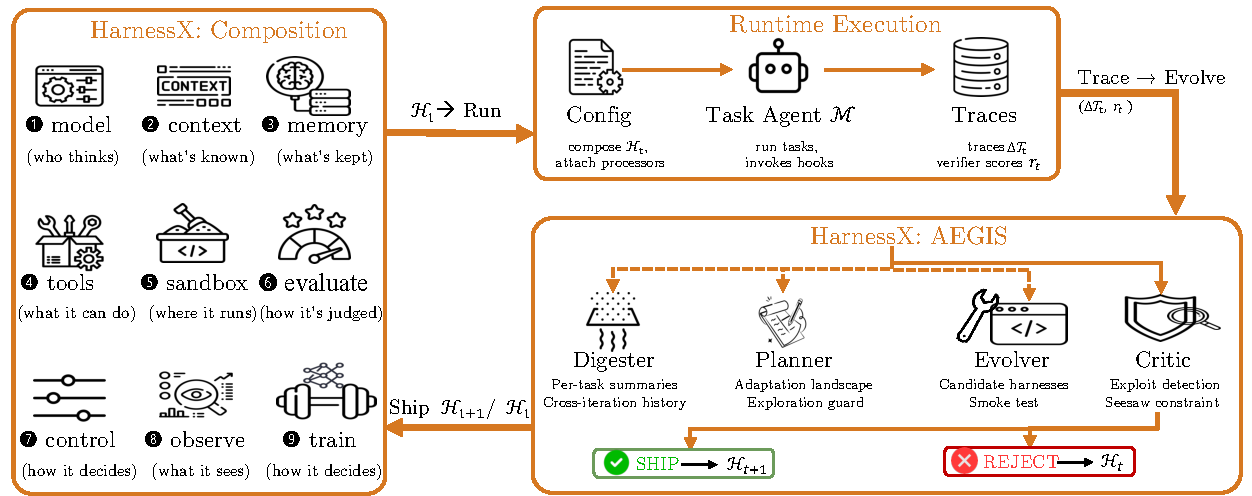
\includegraphics[width=0.82\linewidth]{images/Harness_Evolution.pdf}
  \caption{AEGIS 演化循环。单个元智能体 $\mathcal{M}$ 驱动四个阶段（Digester、Planner、Evolver、Critic），并依据是否存在足够信号，有选择地调用各阶段。确定性门控决定发布或拒绝候选编辑。}
  \label{fig:aegis-loop}
\end{figure}

\subsection{操作镜像}
\label{sec:aegis-mirror}

我们把 harness 演化形式化为符号产物上的马尔可夫决策过程（MDP）。表~\ref{tab:operational-mirror} 总结了这一映射；下面先给出三个奠定对应关系的定义。

\paragraph{定义 1（Harness 配置）。}
Harness 配置是一个元组 $\mathcal{H}=(c_1,c_2,\ldots,c_9)$，其中每个 $c_i\in\mathcal{C}_i$ 实例化九个行为维度（第~\ref{sec:foundry-taxonomy} 节）之一：模型选择（$c_1$）、上下文组装（$c_2$）、记忆管理（$c_3$）、工具生态（$c_4$）、执行环境（$c_5$）、评估与奖励（$c_6$）、控制与安全（$c_7$）、可观测性（$c_8$）以及训练桥梁（$c_9$）。每个 $\mathcal{C}_i$ 是第 $i$ 维有效处理器配置的集合，受钩子类型契约和单例组排斥约束（第~\ref{sec:foundry-processor} 节）。

\paragraph{定义 2（Harness 编辑）。}
Harness 编辑是函数 $e:\mathcal{H}\to\mathcal{H}$，它修改一个或多个维度，同时保持类型契约。动作空间 $\mathcal{E}$ \textit{离散但开放}：每项编辑都是由元智能体大语言模型生成的代码级产物（新的处理器源码、修改后的提示词模板、重新配置的工具注册表或控制流重写），而不是从预先枚举的集合中选择。系统并非通过穷举搜索来控制组合爆炸，而是利用大语言模型的生成能力——Planner 根据轨迹支撑的假设提出编辑——并由类型约束在生成时剪除无效组合。

\paragraph{定义 3（操作镜像）。}
操作镜像是元组 $(\mathcal{H},\mathcal{E},\mathcal{R},\mathcal{T})$，其中 $\mathcal{H}$ 是 harness 配置空间（状态），$\mathcal{E}$ 是代码级编辑空间（动作），$\mathcal{R}:\mathcal{H}\times\mathcal{E}\to\mathbb{R}$ 把配置--编辑对映射为标量奖励（适配批次上聚合的验证器得分），$\mathcal{T}$ 则是提供超越标量信号之结构化反馈的轨迹存储。该元组在 harness 层形成 MDP：harness 配置是状态，带类型的编辑是动作，执行轨迹与验证器得分构成反馈，而确定性接受门控控制状态转移。

\paragraph{MDP 实例化。}
令 $\mathcal{H}_t$ 表示第 $t$ 次迭代的 harness 配置（整个演化过程中模型 $\mathcal{M}$ 固定），令 $\mathcal{T}_t$ 表示此前所有执行所累积的轨迹存储。我们把符号状态定义为 $s_t=(\mathcal{H}_t,\mathcal{T}_t)$。Harness 更新策略 $\pi_{\mathrm{evo}}$ 选择动作 $a_t\sim\pi_{\mathrm{evo}}(\cdot\mid s_t)$，其中 $a_t\in\mathcal{E}$ 是从构建器代数中抽取的一项代码级编辑。应用该编辑得到候选 harness $\widetilde{\mathcal{H}}_t=a_t(\mathcal{H}_t)$。使用固定模型 $\mathcal{M}$ 在适配批次上运行候选方案，会产生新轨迹 $\Delta\mathcal{T}_t$ 和逐任务验证器得分 $r_t$。确定性接受算子 $U(\widetilde{\mathcal{H}}_t,\mathcal{T}_t,r_t)$ 随后提交候选方案（$\mathcal{H}_{t+1}=\widetilde{\mathcal{H}}_t$）或拒绝它（$\mathcal{H}_{t+1}=\mathcal{H}_t$），并执行跷跷板约束：候选方案不得使 $\mathcal{T}_t$ 中记录的任何先前已解决任务退化。无论接受还是拒绝，轨迹存储都会增长：$\mathcal{T}_{t+1}=\mathcal{T}_t\cup\Delta\mathcal{T}_t$。

该 MDP 运行在 harness 层：在单项任务内部，$\mathcal{H}_t$ 与固定模型 $\mathcal{M}$ 共同决定智能体行为；跨迭代时，harness 更新策略 $\pi_{\mathrm{evo}}$ 修改 harness。AEGIS 把 $\pi_{\mathrm{evo}}$ 实现为四阶段流水线（Digester、Planner、Evolver、Critic），通过轨迹压缩、适配规划、编辑生成和候选评估，把 $s_t$ 映射为候选编辑。

\subsection{符号空间中的病态现象}
\label{sec:aegis-pathologies}

操作镜像并非单纯类比；它把强化学习概念转化为设计需求。我们把强化学习中有充分文献记载的三种失败模式——奖励黑客~\cite{guo2025deepseek}、灾难性遗忘~\cite{kirkpatrick2017overcoming} 和探索不足~\cite{ladosz2022exploration}——统称为\textit{强化学习病态现象}。Harness 适配一旦被构造为符号产物上的 MDP，这些病态现象就会以放大的形式重新出现，其形态由符号环境的两个属性决定：（1）语言模型 Evolver 能够构造数值参数扰动无法表达的结构化漏洞利用；（2）对共享组件的编辑会通过 harness 非局部传播。下述每种病态现象都促成了第~\ref{sec:aegis-arch} 节中的一项对应架构防御。

\paragraph{奖励黑客。}
在标准强化学习中，奖励黑客~\cite{guo2025deepseek} 利用奖励信号中的漏洞，却并未真正完成任务。符号 harness 演化会放大这一风险，因为 Evolver 可以直接针对验证协议：把基准答案嵌入提示词、利用验证器的格式规律，或引入一个重写输出以匹配验证器预期的处理器。

\paragraph{灾难性遗忘。}
当任务分布某一区域的性能改善却伤害另一区域时，就会发生灾难性遗忘~\cite{kirkpatrick2017overcoming}。在符号 harness 演化中，修复失败模式 $A$ 的编辑可能悄然使模式 $B$ 退化，因为影响会经由共享上下文、工具、记忆策略和控制规则传播。如果没有显式回归检查，只以失败任务轨迹为条件的 Evolver 就无法区分局部增益与全局退化。

\paragraph{探索不足。}
探索不足~\cite{ladosz2022exploration} 表现为偏向低风险局部编辑：改写提示词、调整工具描述或微调控制流。这些编辑生成成本低，而且经常能通过门控而不使已解决任务退化，从而使后续 Planner 的假设继续偏向相同的编辑邻域。结构性变化（把单个智能体分解为多个智能体、替换控制策略或采用新的记忆架构）需要有意识地形成假设，很少会从以轨迹为条件的局部修复中自然产生。如果没有提出超出眼前失败邻域之编辑的机制，局部编辑耗尽后，系统就会进入平台期。

\paragraph{小结。}
符号 harness 演化继承了强化学习的结构性风险（奖励黑客、灾难性遗忘和探索不足）；AEGIS 分别用 Critic、确定性门控层和 Planner 应对这三类风险。

\begin{algorithm}[H]
\small
\caption{AEGIS Harness 演化循环（选择性调用）}
\label{alg:aegis-loop}
\SetAlgoLined
\LinesNumbered
\KwInput{初始 harness $\mathcal{H}_0$，元智能体 $\mathcal{M}$，预算 $T$，耐心值 $P$，阈值 $\alpha$}
\KwOutput{演化后的 harness $\mathcal{H}_{t+1}$，轨迹存储 $\mathcal{T}_{t+1}$}
$\mathcal{T}_0\leftarrow\emptyset$\; $\mathit{idle}\leftarrow0$\;
\For{$t=0,1,\ldots,T{-}1$}{
  采样批次 $B_t$；在 $B_t$ 上运行 $\mathcal{H}_t$，得到轨迹 $\Delta\mathcal{T}_t$；$\mathcal{T}_{t+1}\leftarrow\mathcal{T}_t\cup\Delta\mathcal{T}_t$\;
  \tcc{Digester（选择性）}
  $(\mathit{evidence}_t,a_t)\leftarrow\mathcal{M}.\textsc{Digester}(\Delta\mathcal{T}_t,\mathcal{T}_t)$\;
  \lIf{$a_t<\alpha$}{$\mathcal{H}_{t+1}\leftarrow\mathcal{H}_t$\; $\mathit{idle}{+}{+}$\; \textbf{continue}}
  \tcc{Planner（选择性）}
  $\mathit{landscape}_t\leftarrow\mathcal{M}.\textsc{Planner}(\mathit{evidence}_t)$\;
  \lIf{$\mathit{landscape}_t=\emptyset$}{$\mathcal{H}_{t+1}\leftarrow\mathcal{H}_t$\; $\mathit{idle}{+}{+}$\; \textbf{continue}}
  \tcc{Evolver（选择性）}
  $\{(\widetilde{\mathcal{H}}_t^{\,k},\mathrm{manifest}_k)\}_{k=1}^{K_t}\leftarrow\mathcal{M}.\textsc{Evolver}(\mathcal{H}_t,\mathit{landscape}_t)$\;
  \lIf{$K_t=0$}{$\mathcal{H}_{t+1}\leftarrow\mathcal{H}_t$\; $\mathit{idle}{+}{+}$\; \textbf{continue}}
  \tcc{Critic 与门控（必选）}
  $\mathit{ranking}\leftarrow\mathcal{M}.\textsc{Critic}(\{(\widetilde{\mathcal{H}}_t^{\,k},\mathrm{manifest}_k)\},\mathit{evidence}_t)$\;
  $k^\star\leftarrow\bot$\;
  \ForEach{$\mathit{ranking}$ 中的 $k$}{
    \lIf{\textnormal{DeterministicGate}$(\widetilde{\mathcal{H}}_t^{\,k},\mathcal{H}_t,\mathcal{T}_t)$ 通过}{$k^\star\leftarrow k$\; \textbf{break}}
  }
  \lIf{$k^\star\neq\bot$}{$\mathcal{H}_{t+1}\leftarrow\widetilde{\mathcal{H}}_t^{\,k^\star}$\; $\mathit{idle}\leftarrow0$}
  \lElse{$\mathcal{H}_{t+1}\leftarrow\mathcal{H}_t$\; $\mathit{idle}{+}{+}$}
  \lIf{$\mathit{idle}\geq P$}{\textbf{break}}
}
\Return $\mathcal{H}_{t+1},\mathcal{T}_{t+1}$
\end{algorithm}

\subsection{AEGIS 架构}
\label{sec:aegis-arch}

AEGIS 是 \ProjectName 的 harness 演化引擎。它由按预定义工作流排列的四个阶段组成——Digester、Planner、Evolver、Critic——并全部由同一个元智能体大语言模型驱动，由该模型\textit{选择性调用}各阶段：没有外部路由器决定是否执行某个阶段，而是元智能体本身在每个阶段判断是否有足够信号继续。Digester、Planner 和 Evolver 各自评估继续条件，并可能令本轮短路（可操作性低于阈值、适配图景为空或没有可行候选方案）；任何到达 Critic 的候选方案则都必须经过 Critic 与确定性门控层。未经 Critic 和门控，任何编辑都不能发布。四阶段分工对应第~\ref{sec:aegis-pathologies} 节的病态现象：Digester 把原始轨迹压缩为结构化的任务级证据；Planner 构建同时覆盖渐进式与结构性变化的适配图景；Evolver 生成带显式变更清单的带类型构建器编辑；Critic 与门控层则拒绝那些所声称改善缺乏轨迹支持，或在接受后会使先前已解决任务退化的编辑。

所有阶段共享同一个信息底座：轨迹存储，即执行事件、经验证器评分的结果、回归信号，以及已发布或被拒编辑的结构化记录。除轨迹存储和当前 harness $\mathcal{H}_t$ 外，任何阶段都不消费其他输入。数据通过带选择性门控的流水线向前流动：Digester 可能判定不存在可操作的失败（所有任务均通过，或信号过于稀疏），并立即终止本轮；Planner 可能根据当前证据与编辑历史找不到可行的适配图景；Evolver 也可能无法产出类型安全的候选方案。在这些情况下，本轮都会以空操作干净退出。只有 Critic 和确定性门控是无条件环节：任何从上游阶段存活下来的候选方案都必须通过二者才能发布。Critic 还可以向 Evolver 发出一次修订请求，再给出最终裁决。

\paragraph{Digester。}
GAIA 上的一次迭代（103 个任务，pass@2）会产生约 1000 万个原始轨迹 token，包括模型推理步骤、工具调用及其输出和计时元数据。把如此大体量的内容直接交给下游阶段会超出上下文限制，而朴素截断又会丢失诊断信号。Digester 把每个任务的轨迹压缩为结构化的逐任务摘要：二元结果、失败类别（若有）、涉及的组件标识符，以及支持证据片段。它还提供跨迭代连续性：每个任务摘要都链接到其先前结果与已发布编辑的历史，让 Planner 能够区分持续性失败与瞬时噪声。

\paragraph{Planner。}
Planner 接收 Digester 的输出（带跨迭代历史的任务级摘要），并构建适配图景：哪些任务失败、尝试过哪些编辑、涉及哪些组件，以及哪些编辑类型（提示词、工具、处理器、配置）尚未尝试。该阶段是防御探索不足的主要机制：先构建图景、后生成编辑，能够防止流水线收敛到以轨迹为条件的局部修复，并确保在考虑渐进式提示词编辑的同时，也考虑结构性变化（增加工具、重写处理器、重新设计记忆策略）。

\paragraph{Evolver。}
给定 Planner 的适配图景，Evolver 生成一个或多个候选 harness $\{\widetilde{\mathcal{H}}_t^{\,k}\}_{k=1}^{K_t}$，每个候选方案都表示为当前 harness $\mathcal{H}_t$ 上的一项带类型构建器操作。每个候选方案均带有\textit{变更清单}：被编辑的组件、预期行为效果，以及预计改善或退化的任务。引入新的处理器代码时，Evolver 还必须提供冒烟测试，确认处理器能够实例化并在合成输入上运行且不抛出异常。构建器代数保证类型安全（每个候选方案都满足钩子类型契约和处理器组合规则），但不保证行为安全；通过类型检查的编辑仍可能产生非局部行为影响，而这些影响只有 Critic 与门控层能够检测。

\paragraph{Critic 与门控。}
Critic 防御奖励黑客，确定性门控层防御灾难性遗忘。Critic 把每个候选方案的变更清单与轨迹证据进行比较，评估编辑是否会通过共享状态或控制流引发非局部影响。发现缺口时，它会向 Evolver 发出一次修订请求。经过至多一次修订循环后，Critic 返回 \texttt{no\_op} 或有序的 \texttt{ship\_ranking}。确定性门控随后依次执行接受检查：清单完整性、配置规范化（确保候选方案处于规范形式）、构建或冒烟测试（适用时），以及跷跷板约束（对先前已通过任务进行回归检查；第~\ref{sec:aegis-mirror} 节）。第一个失败的检查会中止后续序列；通过的候选方案被提交，失败的候选方案则连同拒绝原因一起归档。这种设计把大语言模型判断与接受决定解耦：不论 Critic 如何建议，最终只有确定性检查能决定是否发布。

\paragraph{设计原则。}
语言模型子智能体负责探索、提出假设和建议；带类型结构与确定性门控决定哪些内容能够发布。这种分离确保，无论大语言模型子智能体出现何种失败模式，安全属性（无回归、无未经审计的编辑）都能成立。

\subsection{适配循环}
\label{sec:aegis-loop}

算法~\ref{alg:aegis-loop} 形式化了适配循环（每次迭代对应第~\ref{sec:experiments} 节中的一“轮”）。从初始 harness $\mathcal{H}_0$ 出发，每次迭代都在适配批次上执行当前 harness，并选择性调用四个阶段：Digester、Planner 和 Evolver 分别根据继续条件（足够的可操作性、非空图景和至少一个类型安全候选方案）进行门控，而任何抵达 Critic 与确定性门控的候选方案都必须经过这两者。只有候选方案通过全部接受检查，本轮才会提交新的 harness。

\subsection{通过集成路由实现变体隔离}
\label{sec:aegis-ensemble}

适配循环（第~\ref{sec:aegis-loop} 节）维护单一 harness $\mathcal{H}_t$。当任务需要相互冲突的行为时，改善一个子集的编辑可能使另一个子集退化；跷跷板约束会拒绝该编辑，从而保护稳定性，却也丢弃了局部有益的变更。\textit{变体隔离}维护至多 $K$ 个 harness 变体 $\{\mathcal{H}_t^{(1)},\ldots,\mathcal{H}_t^{(V_t)}\}$（$V_t\leq K$），并依据此前各轮中各变体在相应任务簇上的估计成功率，把每项任务路由到成功率最高的变体，从而解除这一限制。我们称该机制为\textit{集成路由}。

门控层为每个候选方案区分两种结果：（1）编辑改善部分任务而不使任何任务退化，此时将其应用于目标变体；（2）编辑改善一个子集但使其他任务退化，此时系统不会直接拒绝编辑，而是派生一个新变体（若池已满，则淘汰性能最低的变体）。一旦存在多个变体，跷跷板约束就限定在逐变体范围：针对变体 $k$ 的候选方案只在路由到 $k$ 的任务上测试，因此对一个任务簇的改善不会使另一任务簇退化。该设计预测了三个属性，并在第~\ref{sec:exp-strategy} 节得到验证：（1）聚合轨迹不退化（峰值 $=$ 最终值）；（2）更多轮次中持续探索；（3）总 token 消耗更低。

\section{Harness--模型协同演化}
\label{sec:method-coevolution}

第~\ref{sec:method-foundry} 节和第~\ref{sec:method-aegis} 节表明，在基础模型保持固定时，仅演化 harness 已能带来显著收益，而且对于更弱、更小的任务智能体，这些收益最大，因为更好的 harness 最容易弥补它们的行为缺口。协同演化并不取代这条路线，而是沿第二个轴扩展它。对于能力受限的小模型，harness 演化最终会触及\textit{脚手架上限}：harness 一旦提供了正确的工具、上下文和控制流，约束因素就变成冻结模型能否真正利用它们；harness 编辑无法提供模型本身所缺乏的推理能力。

对称地，在固定 harness 下训练模型会遇到\textit{训练信号上限}：如果脚手架从未呈现能够激发新能力的上下文、工具或控制流，新获得的能力便得不到运用。模型是智能体的\textit{认知核心}，负责推理和规划；harness 是其\textit{执行装置}，决定模型感知什么、能调用什么，以及执行受到哪些约束。更精良的装置不能弥补薄弱的核心，更强大的核心也无法弥补从不调用它的装置。协同演化正是针对这一瓶颈：在演化 harness 的同一循环内训练模型，让智能体同时沿两个轴改进，从而突破任一单独改进都会留下的上限。共同演化互补能力组件的原则也见于其他场景：K\textsuperscript{2} Agent~\cite{wu2026k} 协同演化“知其然”（陈述性知识）与“知其所以然”（程序性技能），用于分层移动设备控制。

图~\ref{fig:coevolution-loop} 展示了协同演化机制。\ProjectName 并非在彼此独立的 harness 演化阶段和模型训练阶段之间交替，而是在单次迭代中基于共享回放缓冲区同时运行二者。我们将形式化该迭代（第~\ref{sec:coevolution-loop} 节），描述两种优化底座（第~\ref{sec:coevolution-dual-grpo} 节），通过跨 harness GRPO 说明模型训练目标（第~\ref{sec:coevolution-grpo} 节），并刻画共享缓冲区上的离策略训练（第~\ref{sec:coevolution-offpolicy} 节）；正是后一性质让模型强化学习不产生额外的 rollout 成本。

\begin{figure*}[!htbp]
  \centering
  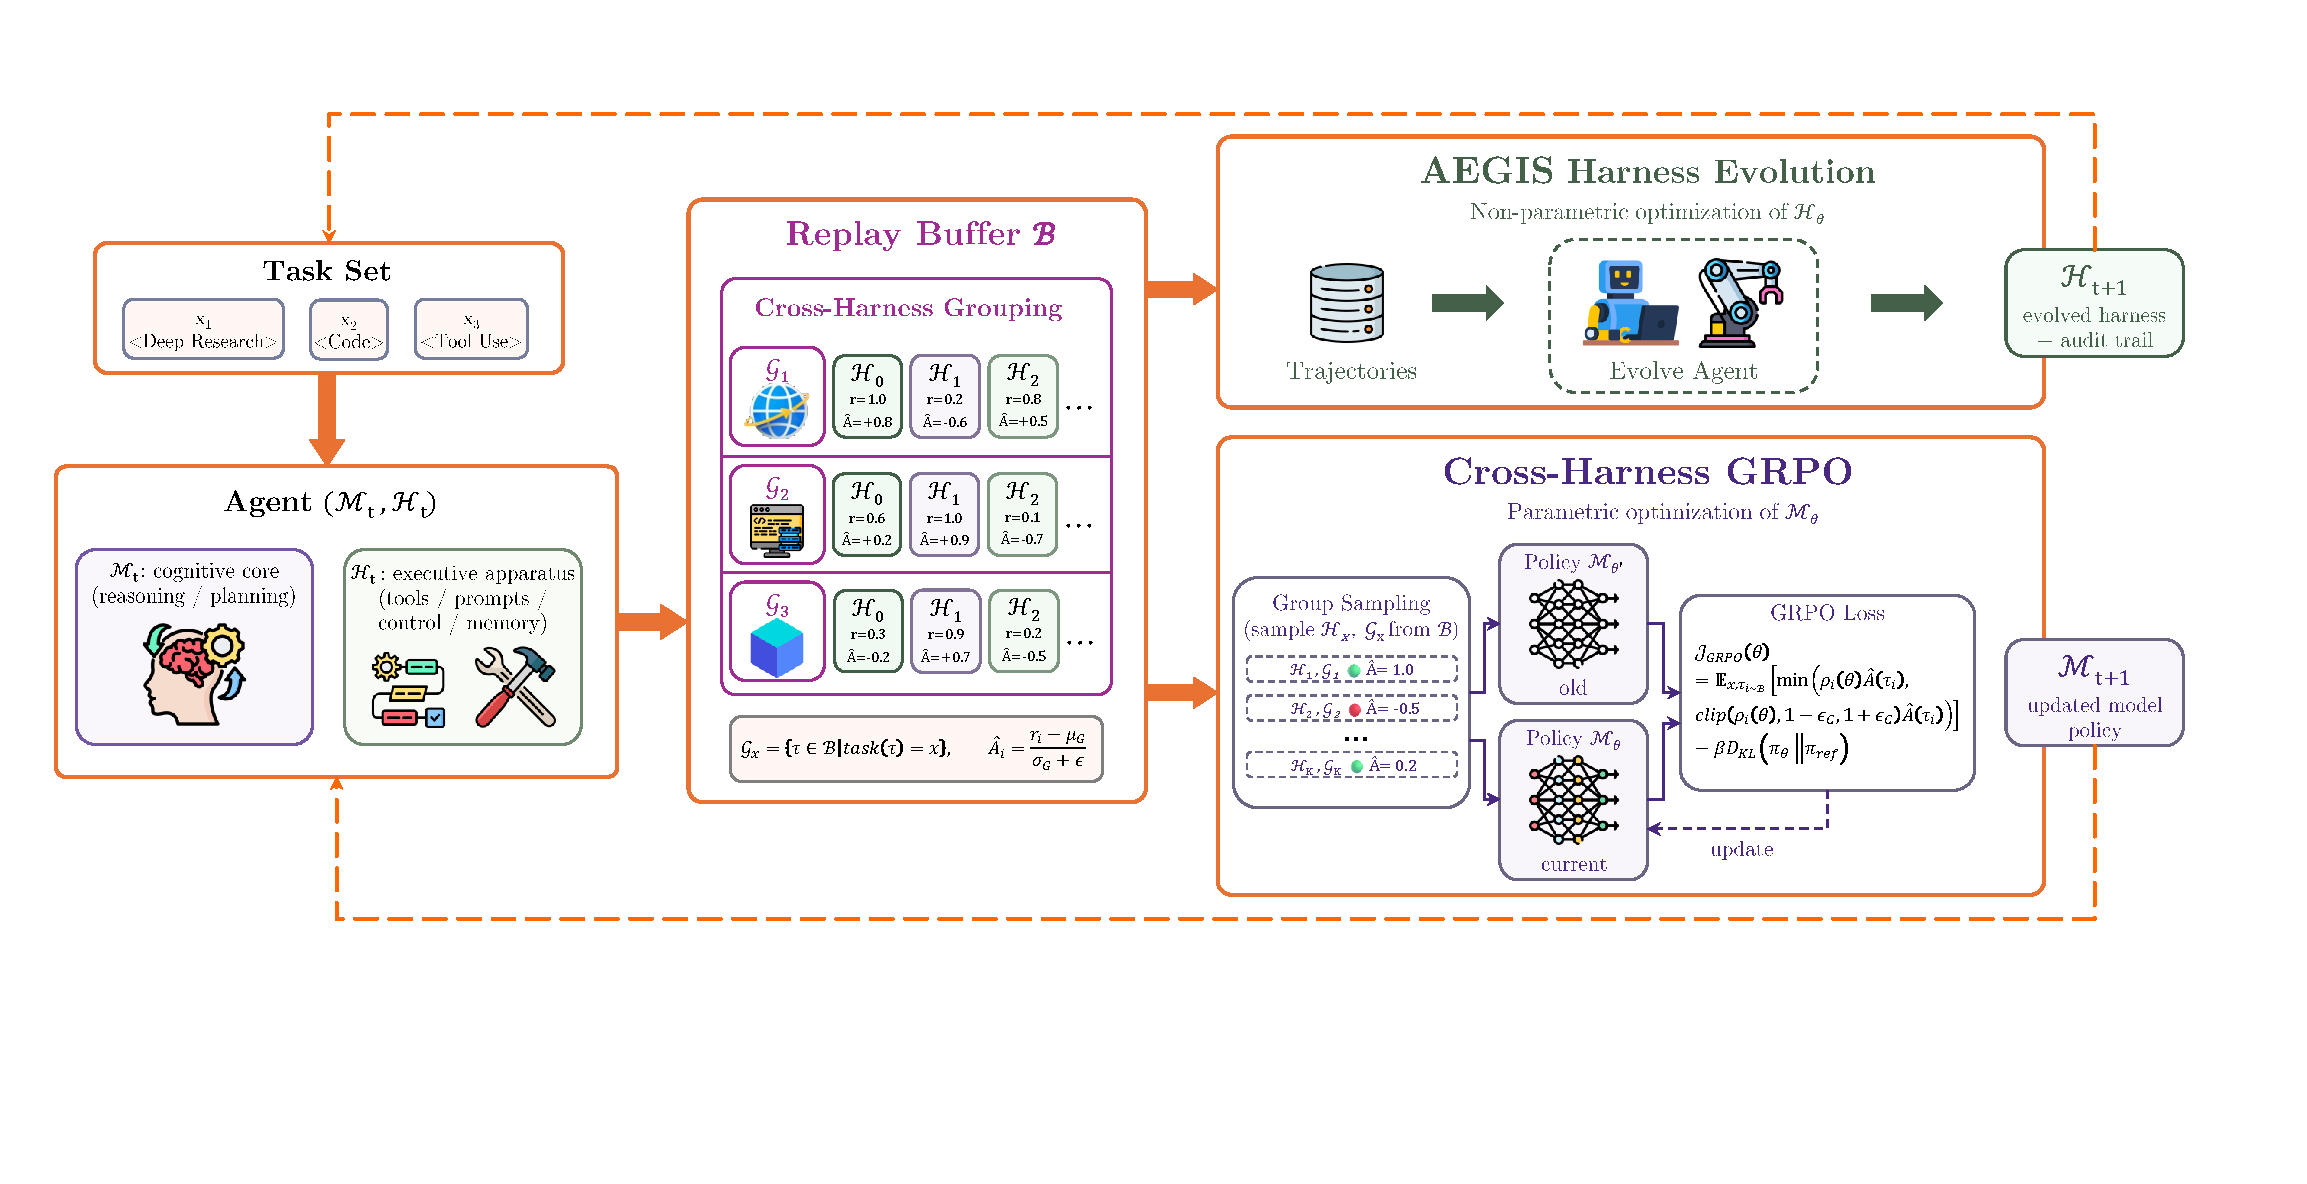
\includegraphics[width=\textwidth]{images/co-evo.pdf}
  \caption{\textbf{Harness--模型协同演化循环。}智能体 $(\mathcal{M}_t,\mathcal{H}_t)$ 在固定验证器和可观测性层下运行任务批次 $B_t$；所得轨迹与奖励 $(\tau,r)$ 进入共享回放缓冲区 $\mathcal{B}$。跨 harness 分组把同一任务在不同 harness 版本下的轨迹汇集起来，并计算组相对优势 $\hat{A}$。同一缓冲区以相同数据驱动两项更新：AEGIS harness 演化（Digester $\to$ Planner $\to$ Evolver $\to$ Critic，产生演化后的 harness $\mathcal{H}_{t+1}$）和\textbf{跨 harness GRPO}（组采样与裁剪 GRPO 目标，产生更新后的模型 $\mathcal{M}_{t+1}$）；二者共同进入下一次迭代。}
  \label{fig:coevolution-loop}
\end{figure*}

\subsection{协同演化迭代}
\label{sec:coevolution-loop}

协同演化作用于二元组 $(\mathcal{M}_t,\mathcal{H}_t)$，其中 $\mathcal{M}_t$ 表示可训练模型参数（放宽第~\ref{sec:method-aegis} 节中的冻结模型假设），$\mathcal{H}_t$ 表示第 $t$ 次迭代的 harness 配置。系统维护采用先进先出淘汰策略、容量固定的回放缓冲区 $\mathcal{B}$。每次迭代按如下步骤进行：

\begin{enumerate}[leftmargin=*]
  \item \textbf{Rollout。}在适配批次 $B_t$ 上运行 $(\mathcal{M}_t,\mathcal{H}_t)$；可观测性层把每个 episode 记录为完整轨迹 $\tau_i$，涵盖每轮模型输出、每次工具调用和每项工具结果。
  \item \textbf{验证。}固定验证器把每条轨迹评分为标量奖励 $r_i$。保持验证器不变，可使不同 harness 版本间的奖励保持可比，这是跨 harness 优势（式~\ref{eq:grpo-advantage}）的必要条件。
  \item \textbf{写入缓冲区。}把每条已评分轨迹连同生成它的 harness 版本追加到共享缓冲区 $\mathcal{B}$，使连续各轮累积而非覆盖；先进先出淘汰确保 $\mathcal{B}$ 仅保留最近若干轮。
  \item \textbf{Harness 演化}（$\mathcal{H}_{t+1}\leftarrow\text{AEGIS}(\mathcal{H}_t,\mathcal{B})$，非参数，第~\ref{sec:method-aegis} 节）。元智能体读取缓冲轨迹，将其视为脚手架失败位置的证据，提出一项离散结构编辑，并且仅在 Critic 和门控层验证通过后接纳该编辑。
  \item \textbf{行为对数概率。}对本轮刚加入的轨迹，在其生成模型 $\mathcal{M}_t$ 下执行一次前向传播，得到 token 级对数概率 $\pi_{\theta_{\text{old}}}(\tau_i)$ 并缓存，以用于 GRPO 损失；更早轮次的轨迹复用它们写入时缓存的数值（第~\ref{sec:coevolution-offpolicy} 节）。
  \item \textbf{GRPO 更新}（$\mathcal{M}_{t+1}\leftarrow\text{GRPO}(\mathcal{M}_t,\mathcal{B})$，参数化，第~\ref{sec:coevolution-grpo} 节）。把轨迹划分为跨 harness 版本的逐任务组，为每条轨迹分配组相对优势，并执行带固定参考模型 KL 锚点的裁剪策略梯度步骤。
  \item \textbf{推进。}携带演化后的二元组 $(\mathcal{M}_{t+1},\mathcal{H}_{t+1})$ 返回步骤 1。
\end{enumerate}

每条轨迹同时充当 AEGIS 的诊断证据与 GRPO 的训练信号。Harness 演化（步骤 4）和模型更新（步骤 5--6）读取同一缓冲区，但在同一次迭代内，二者都不以另一方的输出为条件；必须等两者全部完成，下一轮 rollout 才会开始。

\subsection{优化底座}
\label{sec:coevolution-dual-grpo}

\paragraph{Harness 侧（非参数优化）。}
Harness 演化遵循第~\ref{sec:method-aegis} 节的方法，并从回放缓冲区 $\mathcal{B}$ 提取轨迹证据。它与独立运行 AEGIS 的主要区别是，$\mathcal{B}$ 包含来自多个模型检查点 $\mathcal{M}_0,\mathcal{M}_1,\ldots,\mathcal{M}_t$ 的轨迹，因此 Digester 所观察的行为变化同时来自模型更新与 harness 编辑。

\paragraph{模型侧（通过 GRPO 进行参数优化）。}
关键设计选择是\textit{跨 harness 分组准则}（在第~\ref{sec:coevolution-grpo} 节形式化）：共享同一任务标识符的所有轨迹组成一个 GRPO 组，不论它们由哪个 harness 或模型检查点产生，因此组内差异主要反映策略差异，而不只是采样噪声。

\paragraph{互补性。}
Harness 更新执行参数更新无法表达的离散结构变更（增加工具、替换控制处理器、重构提示词）。模型更新执行依赖高维上下文状态、无法由符号规范刻画的细粒度行为调整（何时调用哪个工具、如何表述查询、何时终止）。Harness 定义粗粒度的策略架构，模型则学习如何利用它。

\subsection{通过跨 Harness GRPO 训练模型}
\label{sec:coevolution-grpo}

我们采用组相对策略优化（GRPO）~\cite{shao2024deepseekmath}。形式化地，缓冲区中的每条轨迹按如下方式生成：
\begin{equation}
  \tau_i\sim\text{Agent}(\mathcal{M}_k,\mathcal{H}_k,x_i),\quad k\in\{0,1,\ldots,t\},
  \label{eq:trajectory-generation}
\end{equation}
其中 $i$ 是缓冲区 $\mathcal{B}$ 中的 $(x,\tau)$ 索引，$\mathcal{M}_k$ 和 $\mathcal{H}_k$ 是把任务 $x_i$ rollout 为轨迹 $\tau_i$ 时使用的模型检查点与 harness。由于先进先出淘汰把缓冲区限制在最近若干次迭代，缓冲轨迹来自与当前策略相近的模型版本。然而，它们的策略（工具选择、提示词结构、控制流逻辑）差异显著，而这种多样性来自连续多个 harness 版本 $\mathcal{H}_0,\ldots,\mathcal{H}_t$。在单策略强化学习中，组内变化仅来自随机采样；这里的变化则主要由 harness 身份决定，因此跨 harness 分组准则（式~\ref{eq:cross-harness-group}）对于有意义的优势估计至关重要。

形式化地，对于任务 $x$，轨迹组会收集 $x$ 的全部轨迹，不论它们由哪个 $(\mathcal{M}_k,\mathcal{H}_k)$ 对产生：
\begin{equation}
  \mathcal{G}_x=\{\tau_i\in\mathcal{B}\mid\text{task}(\tau_i)=x\}
  =\bigcup_k\{\tau\sim\text{Agent}(\mathcal{M}_k,\mathcal{H}_k,x)\}.
  \label{eq:cross-harness-group}
\end{equation}
因此，模型接收的梯度信号来自策略之间的奖励对比，而不是固定策略内部的随机变化，从而能够内化不同 harness 版本中成功的策略。

\paragraph{任务级对齐，而非动作级对齐。}
跨 harness GRPO 执行\textit{任务级}对齐：来自不同 harness 版本的轨迹按任务身份分组，只依据验证器奖励比较。它不要求动作级对齐，因此动作空间不兼容（工具模式、提示词结构或控制流处理器不同）的 harness 版本可以在同一组中共存而不冲突。计算策略梯度时，每条轨迹 $\tau_i$ 都在生成它的 harness 版本 $\mathcal{H}_k$ 下回放：模型的对数概率 $\pi_\theta(\tau_i\mid x)$ 针对 $\mathcal{H}_k$ 在每一轮本应构造的提示词、工具模式和观察上下文进行评估。因此，GRPO 梯度完全作用于以 harness 专用上下文为条件的模型输出 token，而不作用于 harness 结构动作或环境转移。这种设计把 harness 演化（可以在不同版本间自由修改动作空间）与模型训练（只要求在每条轨迹自己的 harness 上下文中得到 token 级对数概率）解耦。

组相对优势为：
\begin{equation}
  \hat{A}(\tau_i)=\frac{r_i-\mu(\mathcal{G}_x)}{\sigma(\mathcal{G}_x)+\epsilon},
  \label{eq:grpo-advantage}
\end{equation}
其中 $r_i$ 是轨迹 $\tau_i$ 的奖励，$\mu(\mathcal{G}_x)$ 和 $\sigma(\mathcal{G}_x)$ 分别是组内奖励均值和标准差。不断演化的 harness 相当于模型强化学习的结构化探索算子：每个新版本都向任务的采样分布注入一种不同的行为模式，式~\ref{eq:grpo-advantage} 中的优势则把模型推向验证器评分最高的模式。因此，单策略采样无法提供的探索广度由不断演化的脚手架自身提供。

需要最大化的策略目标为：
\begin{equation}
  \mathcal{J}_{\text{GRPO}}(\theta)=\mathbb{E}_{x,\,\tau_i\sim\mathcal{B}}\!\left[\min\!\left(\rho_i(\theta)\hat{A}(\tau_i),\;\text{clip}\!\left(\rho_i(\theta),1{-}\epsilon_c,1{+}\epsilon_c\right)\hat{A}(\tau_i)\right)\right]-\beta D_{\text{KL}}\!\left(\pi_\theta\,\|\,\pi_{\text{ref}}\right),
  \label{eq:grpo-objective}
\end{equation}
其中
\begin{equation}
  \rho_i(\theta)=\frac{\pi_\theta(\tau_i\mid x)}{\pi_{\theta_{\text{old}}}(\tau_i\mid x)},\qquad \pi_{\theta_{\text{old}}}=\mathcal{M}_d,
  \label{eq:grpo-ratio}
\end{equation}
是当前策略 $\mathcal{M}_k$ 与生成 $\tau_i$ 的检查点 $\mathcal{M}_d$（式~\ref{eq:trajectory-generation}）之间的重要性采样比，$\epsilon_c$ 是裁剪阈值，$\beta D_{\text{KL}}(\pi_\theta\|\pi_{\text{ref}})$ 则惩罚与固定参考模型 $\pi_{\text{ref}}$ 的偏离。比率中的行为策略 $\pi_{\theta_{\text{old}}}$ 与 KL 项中的参考策略 $\pi_{\text{ref}}$ 不同：$\pi_{\text{ref}}=\mathcal{M}_0$ 在整个训练过程中固定，而 $\pi_{\theta_{\text{old}}}$ 随轨迹变化，必须从缓冲区恢复（第~\ref{sec:coevolution-offpolicy} 节）。

\subsection{混合策略缓冲区上的离策略训练}
\label{sec:coevolution-offpolicy}

回放缓冲区在本质上是离策略的：第 $t$ 次迭代时，其中包含模型检查点 $\mathcal{M}_0,\mathcal{M}_1,\ldots,\mathcal{M}_t$ 在 harness $\mathcal{H}_0,\mathcal{H}_1,\ldots,\mathcal{H}_t$ 下生成的轨迹（式~\ref{eq:trajectory-generation}），所以缓冲区分布与正在更新的策略 $\pi_\theta$ 不匹配。为每条缓冲轨迹恢复 $\pi_{\theta_{\text{old}}}$ 是核心离策略难题。

\paragraph{行为策略 $\pi_{\theta_{\text{old}}}$。}
重要性比率（式~\ref{eq:grpo-ratio}）校正 $\pi_\theta$ 与生成 $\tau_i$ 的检查点 $\mathcal{M}_k$ 之间的差距。由于缓冲区中的 $\mathcal{M}_k$ 各不相同，不能从任何单一模型恢复 $\pi_{\theta_{\text{old}}}(\tau_i)$：我们在写入缓冲区时，于 $\mathcal{M}_k$ 下执行一次前向传播将其物化，把 token 级对数概率缓存在磁盘上，并在每次梯度步骤中复用。这样，缓存的行为对数概率就与每一步重新计算的当前对数概率 $\pi_\theta(\tau_i)$ 解耦。

\paragraph{有界离策略偏差。}
先进先出淘汰把缓冲区限制为 $C$ 条轨迹；若每轮有 $s$ 个样本，最大模型版本滞后为 $\lfloor C/s\rfloor$ 轮，因此每个缓存的 $\pi_{\theta_{\text{old}}}$ 都来自 $\pi_\theta$ 的一个有界窗口之内，生成轨迹的策略不会与正在更新的策略相差过大。同一窗口也限制了 harness 陈旧度，因此跨 harness 组（式~\ref{eq:cross-harness-group}）只混合近期脚手架版本，模型不会主要针对过时 harness 进行训练。

\paragraph{不增加 rollout 成本的回放复用。}
智能体强化学习的主要成本是 rollout（让智能体在环境中执行，包括模型解码、工具调用和验证），而不是梯度更新。在协同演化中，单轮探索只产生一组轨迹，却同时服务于两项更新：相同轨迹既驱动 AEGIS harness 更新（第~\ref{sec:method-aegis} 节），也通过共享缓冲区（第~\ref{sec:coevolution-loop} 节）驱动跨 harness GRPO 模型更新。GRPO 通过回放消费这些轨迹，自身不发起 rollout。因此，加入模型更新的边际成本仅限于：（i）每条轨迹执行一次缓存 $\pi_{\theta_{\text{old}}}$ 的前向传播；（ii）梯度步骤本身，二者都不涉及 rollout。没有哪条轨迹是专为训练模型而生成的。因此，联合优化具有经济性：它只付出离线训练计算的代价，就能获得模型改进，而不增加 harness 演化已经执行的 rollout。

\section{实验}
\label{sec:experiments}

我们从五个方面评估 \ProjectName：跨基准与模型家族的总体有效性（第~\ref{sec:exp-main} 节）、变体管理策略对稳定性的影响（第~\ref{sec:exp-strategy} 节）、Evolver 架构相对于基础设施的贡献（第~\ref{sec:exp-meta-agent} 节）、模型--harness 联合协同演化的收益（第~\ref{sec:exp-coevolution} 节），以及对预测失败模式的实证确认（第~\ref{sec:exp-failure} 节）。

\subsection{实验设置}
\label{sec:exp-setup}

\paragraph{基准。}
如表~\ref{tab:benchmarks} 所示，我们在五个基准上评估，覆盖多步检索、具身规划、网页交互、多轮对话和软件工程。除非另有说明，每项实验最多运行 $T{=}15$ 轮演化；若连续 $P{=}3$ 轮都没有发布编辑，则提前停止。每轮都评估完整任务集，不进行子采样。元智能体 token 预算随基准而异（总计 1 亿至 1.75 亿），但同一基准内不同任务智能体的预算保持不变。

\begin{table}[!htbp]
\centering
\small
\caption{基准特征。}
\label{tab:benchmarks}
\begin{tabular}{llcl}
\toprule
\textbf{基准} & \textbf{领域} & \textbf{采样任务数} & \textbf{验证器} \\
\midrule
GAIA（Level 1--3） & 多步检索 & 103 & 精确匹配 \\
ALFWorld & 具身规划 & 134 & 目标完成 \\
WebShop & 网页交互 & 100 & 属性匹配 \\
$\tau^3$-Bench & 多轮对话 & 3 个领域 & 规则遵循 \\
SWE-bench Verified & 软件工程 & 55 & 补丁解决 \\
\bottomrule
\end{tabular}
\end{table}

\paragraph{模型。}
我们区分两种角色：\textit{元智能体}（除非另有说明，均为 Claude Opus 4.6）驱动 AEGIS 演化循环；\textit{任务智能体}则在演化后的 harness 下运行并解决基准任务。任务智能体涵盖三个家族（Claude Sonnet 4.6、GPT-5.4、Qwen3.5-9B），用于检验单一元智能体能否跨模型家族演化出有效 harness。

\paragraph{基线。}
\textbf{（1）静态 Harness}：由已发表的基准专用提示词与工具定义构建的 \ProjectName 配置，在所有轮次中保持固定。\textbf{（2）Claude Code SDK（CC SDK）}\footnote{Claude Code SDK v0.0.25，\texttt{model="opus"}（Claude Opus 4.6），\texttt{max\_turns=200}。实验于 2026 年 5 月开展。}：一种单智能体 Evolver（每轮一个大语言模型会话），它取代四阶段流水线，但保留相同基础设施和轮次预算，用于把 AEGIS 的多阶段架构与共享基础设施分离（第~\ref{sec:exp-meta-agent} 节）。该基线也可作为 SICA~\cite{robeyns2025self} 等单体 Evolver 的代理。

\paragraph{指标。}
使用基准专用验证器测得的任务成功率（\%）。每轮中每个任务有两次独立尝试（pass@2：任一次成功即视为解决），从而在保留供跷跷板约束使用的逐任务二元信号的同时降低采样噪声；代价是会掩盖低于阈值的成功概率漂移（第~\ref{sec:exp-strategy} 节）。

\paragraph{范围。}
所有报告的增益都在用于演化的同一任务集上测量；本文不评估对未见任务的留出泛化能力。

\begin{figure*}[!htbp]
  \centering
  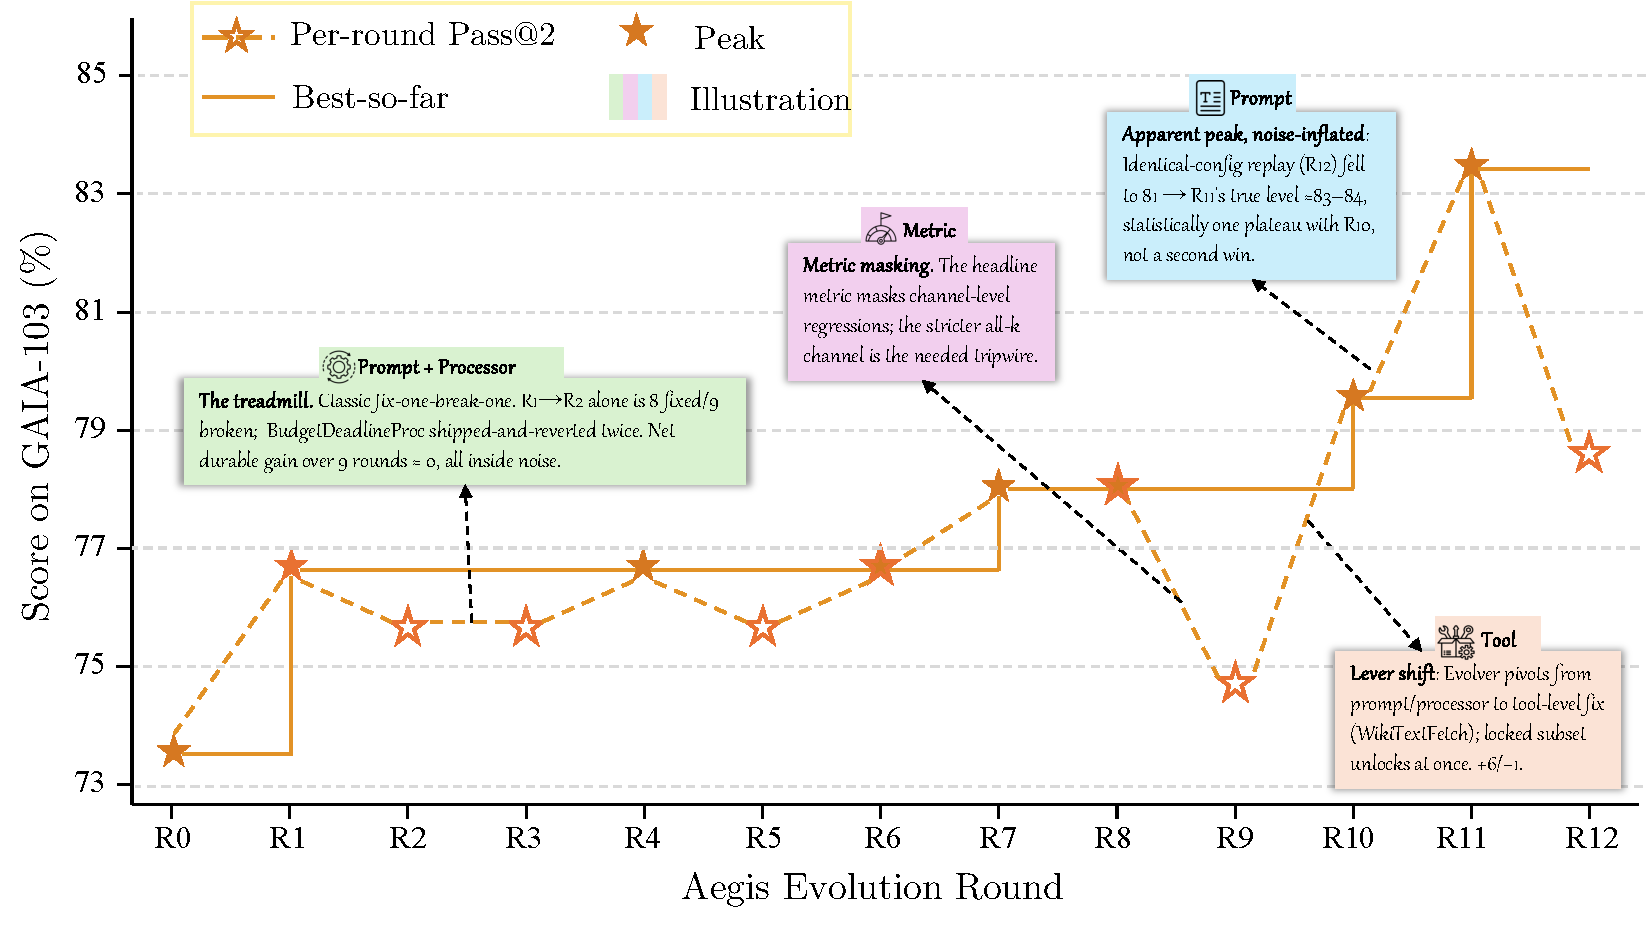
\includegraphics[width=0.85\textwidth]{images/Evolution_Main.pdf}
  \caption{演化轨迹（pass@2 成功率随轮次的变化）。虚线表示静态 harness 基线。}
  \label{fig:evolution-curves}
\end{figure*}

\subsection{主要结果}
\label{sec:exp-main}

表~\ref{tab:main-results} 和图~\ref{fig:evolution-curves} 报告了 harness 演化前后的 pass@2 成功率。AEGIS 改善了 15 个模型--基准配置中的 14 个，平均增益为 $+14.5\%$（最高 $+44.0\%$）。唯一停滞的配置（GAIA、GPT-5.4，$\Delta{=}0.0$）反映了单一 harness 演化在异构任务集上的根本限制；第~\ref{sec:exp-strategy} 节表明，变体隔离可以解决该问题。有一个配置在运行中途退化（$\tau^3$-Bench Telecom，在 R7 为 $-14.0\%$），原因是同类型编辑累积，并在 R9 恢复（第~\ref{sec:exp-failure} 节）。

\begin{table}[!htbp]
\centering
\small
\caption{主要结果（pass@2 成功率，\%）。Evolved 表示达到的峰值准确率；“--”表示领域平均结果，不对应单一峰值轮次。}
\label{tab:main-results}
\resizebox{\textwidth}{!}{%
\begin{tabular}{llcccc}
\toprule
\textbf{基准} & \textbf{任务智能体} & \textbf{初始} & \textbf{演化后} & \textbf{$\Delta$} & \textbf{最佳轮次} \\
\midrule
\multirow{3}{*}{ALFWorld}
  & Claude Sonnet 4.6 & 83.6 & 94.8 & +11.2 & 7 \\
  & GPT-5.4           & 76.9 & \textbf{97.8} & +20.9 & 4 \\
  & Qwen3.5-9B        & 53.0 & 97.0 & +44.0 & 9 \\
\midrule
\multirow{3}{*}{WebShop}
  & Claude Sonnet 4.6 & 60.0 & \textbf{76.0} & +16.0 & 7 \\
  & GPT-5.4           & 55.0 & 73.0 & +18.0 & 8 \\
  & Qwen3.5-9B        & 36.0 & 49.0 & +13.0 & 7 \\
\midrule
\multirow{3}{*}{GAIA}
  & Claude Sonnet 4.6 & 73.8 & \textbf{83.5} & +9.7 & 11 \\
  & GPT-5.4           & 73.8 & 73.8 & 0.0 & 4 \\
  & Qwen3.5-9B        & 20.3 & 37.4 & +17.1 & 4 \\
\midrule
\multirow{3}{*}{SWE-bench Verified}
  & Claude Sonnet 4.6 & 76.4 & \textbf{87.3} & +10.9 & 3 \\
  & GPT-5.4           & 45.5 & 63.6 & +18.2 & 3 \\
  & Qwen3.5-9B        & 23.6 & 41.8 & +18.2 & 2 \\
\midrule
\multirow{3}{*}{$\tau^3$-Bench（平均）}
  & Claude Sonnet 4.6 & 89.6 & \textbf{95.0} & +5.4 & -- \\
  & GPT-5.4           & 76.2 & 90.7 & +14.5 & -- \\
  & Qwen3.5-9B        & 93.5 & 94.6 & +1.1 & -- \\
\bottomrule
\end{tabular}}
\end{table}

\textbf{总体性能。}演化改善了 15 个配置中的 14 个。ALFWorld 上的增益为 $+11.2\%$ 至 $+44.0\%$，WebShop 为 $+13.0\%$ 至 $+18.0\%$，SWE-bench Verified 为 $+10.9\%$ 至 $+18.2\%$。GAIA 上，Sonnet 4.6（$+9.7\%$）和 Qwen3.5-9B（$+17.1\%$）有所改善，而 GPT-5.4 停滞（$\Delta{=}0.0$；修复其失败需要相互冲突的编辑，单一 harness 策略无法兼容）。在 $\tau^3$-Bench 上，GPT-5.4 增益最大（$+14.5\%$）；Qwen3.5-9B 由于其基线已接近上限（$93.5\%$），只提升 $+1.1\%$。

\textbf{与基线性能的反向缩放。}跨基准来看，最弱的任务智能体 Qwen3.5-9B 始终获益最多：ALFWorld 上 $+44.0\%$（基线 $53.0\%$）、GAIA 上 $+17.1\%$（基线 $20.3\%$）、SWE-bench Verified 上 $+18.2\%$（基线 $23.6\%$）。更强的模型 Sonnet 4.6 和 GPT-5.4 在 ALFWorld 上分别提升 $+11.2\%$ 和 $+20.9\%$，在 SWE-bench 上分别提升 $+10.9\%$ 和 $+18.2\%$。例外是 GAIA 上的 GPT-5.4（$\Delta{=}0.0$），其中任务异构性阻止单一 harness 改善聚合准确率——这一观察促成了第~\ref{sec:exp-strategy} 节的变体隔离消融。整体模式表明，较弱模型暴露出更多可由 harness 层编辑弥补的行为缺口；基线性能足够高后，剩余失败越来越需要任务专用适配，而非全局改善。

\textbf{跨模型泛化。}元智能体 Opus 4.6 无需家族专用适配，就能为不同模型家族的任务智能体演化 harness。在 ALFWorld 上，跨家族智能体（GPT-5.4：$+20.9\%$；Qwen3.5-9B：$+44.0\%$）的增益高于同家族智能体（Sonnet 4.6：$+11.2\%$），表明增益大小跟随基线性能，而不是与元智能体模型家族的接近程度。

\textbf{收敛速度跟随失败模式的集中程度。}ALFWorld（GPT-5.4）在 R4 达到峰值，SWE-bench Verified（所有智能体）在 R2--R3 达到峰值；两种情况下，失败都集中在一两类组件上，因此能够快速收敛。GAIA（Sonnet 4.6）需要 11 轮，因为失败横跨四类组件（提示词、工具、处理器、配置），迫使系统依次探索多个编辑邻域。

\paragraph{$\tau^3$-Bench 内部的领域级差异。}
$\tau^3$-Bench 的平均增益掩盖了显著的逐领域差异。GPT-5.4 在 Telecom 上提升 $+25.4\%$（R2 时从 $67.5\%$ 到 $93.0\%$），在 Retail 上提升 $+9.7\%$（R6 时从 $84.2\%$ 到 $93.9\%$）。然而，Sonnet 4.6 在 Telecom 上因同类型编辑累积，在单轮 R7 中退化 $-14.0\%$，并于 R9 恢复（第~\ref{sec:exp-failure} 节）。这揭示了逐编辑门控的结构限制：连续同类型编辑产生的低于阈值耦合会在未被检测的情况下累积，直到越过临界点并触发可见退化。

\paragraph{SWE-bench 上的峰后退化。}
在 SWE-bench Verified（GPT-5.4）上，演化于 R3 达到 $63.6\%$ 的峰值（$+18.2\%$），但到 R5 降为 $50.9\%$（相对峰值 $-12.7\%$）；最终准确率仍比静态基线高 $+5.4\%$。两个因素加速了该基准上的退化：（1）只有 55 个任务，因此每个任务的翻转会使聚合准确率变化约 $1.8\%$（而 $n{=}103$ 时约为 $1.0\%$），更少的退化即可造成可见下降；（2）结构性代码编辑的影响范围比提示词编辑更广。这与 GAIA 上 GPT-5.4 的停滞相呼应：两者都促成了第~\ref{sec:exp-strategy} 节所评估的变体隔离策略。

\subsection{演化策略比较}
\label{sec:exp-strategy}

主要实验（表~\ref{tab:main-results}）使用 Global 策略：在所有任务上演化单一 harness。表~\ref{tab:strategy} 在 GAIA（103 个任务、GPT-5.4、15 轮、AEGIS Evolver）上比较该默认策略与变体隔离策略。

\begin{table}[!htbp]
\centering
\small
\caption{演化策略比较（GAIA、GPT-5.4、AEGIS Evolver、15 轮）。最终值减峰值表示稳定性；负值意味着灾难性遗忘。}
\label{tab:strategy}
\resizebox{\textwidth}{!}{%
\begin{tabular}{lcccc}
\toprule
\textbf{策略} & \textbf{最终（\%）} & \textbf{峰值（\%）} & \textbf{最终$-$峰值} & \textbf{Token 数} \\
\midrule
Ensemble（至多 $K$ 个变体） & \textbf{87.4} & 87.4 & 0.0 & 107.8M \\
Global（单一 harness） & 49.5 & 73.8 & $-24.3$ & 143.7M \\
\bottomrule
\end{tabular}}
\end{table}

\textbf{Global 的失败机制。}Global 策略为全部 103 个任务维护单一 harness。它在 R4 很早就达到 $73.8\%$ 的峰值，随后持续退化：后续编辑引入的回归低于阈值，在 pass@2 二元信号下无法单独检测，却复合成总体下降。峰值--最终差距（$-24.3\%$）远超逐轮二项分布的 $95\%$ 置信区间（$n{=}103$、$p{\approx}0.74$ 时为 $\pm8.5\%$），因此可以排除评估噪声并确认灾难性遗忘（第~\ref{sec:aegis-pathologies} 节）。这解释了表~\ref{tab:main-results} 中 GAIA GPT-5.4 的 $\Delta{=}0.0$ 停滞：Global 无法在该异构任务集上维持改善。

\textbf{Ensemble 为何防止跨变体遗忘。}集成路由维护至多 $K$ 个 harness 变体，并将每项任务路由到先前成功率最高的变体。系统\textit{逐变体}提出和评估编辑，因此改善一个任务簇的编辑不会使另一个任务簇退化。比较结果确认了三个预测属性：（1）聚合轨迹不退化（峰值 $=$ 最终值）；（2）峰值出现更晚（R14 而非 R4），表明持续进行了富有成效的探索；（3）token 消耗更低（107.8M 对 143.7M），因为每项编辑只针对其目标任务簇评估，而非完整任务集；编辑也只作用于分配给它的任务簇，避免退化中的单一 harness 在所有任务上评估时积累无效提议。

\textbf{小结。}变体隔离解决了 Global 下的停滞，把 GAIA GPT-5.4 从 $\Delta{=}0.0$ 提升到 $+13.6\%$（最终 $87.4\%$，无退化）。我们还以试点规模探索了更细粒度的策略（领域感知聚类、任务级锦标赛），但实验只有 30--40 个任务和不超过 8 轮，不足以进行有统计意义的比较。

\subsection{元智能体有效性}
\label{sec:exp-meta-agent}

为解耦 Evolver 架构与基础设施，我们用单智能体 CC SDK Evolver 替换四阶段 AEGIS 流水线，同时共享相同模型（Opus 4.6）、轮次预算和基础设施。两个 Evolver 都在第~\ref{sec:exp-strategy} 节引入的变体隔离下运行，以确保轨迹不退化。表~\ref{tab:meta-agent} 报告 GAIA（103 个任务、GPT-5.4、15 轮）上的比较。

\begin{table}[!htbp]
\centering
\small
\caption{元智能体架构比较（GAIA、GPT-5.4、变体隔离、15 轮）。两个 Evolver 都使用 Opus 4.6。}
\label{tab:meta-agent}
\begin{tabular}{lccc}
\toprule
\textbf{Evolver} & \textbf{准确率（\%）} & \textbf{最佳轮次} & \textbf{Token 数} \\
\midrule
AEGIS & \textbf{87.4} & R14 & 107.8M \\
CC SDK & 86.4 & R12 & 123.1M \\
\bottomrule
\end{tabular}
\end{table}

\textbf{准确率相当，效率不同。}$1.0\%$ 的准确率差距小于一个标准误（$n{=}103$ 时约为 $3.3\%$），说明在这一元智能体能力水平上，四阶段分解并未改善最终准确率。然而，单智能体变体多消耗约 $14\%$ 的 token（123.1M 对 107.8M）。我们把这种差异归因于 Digester 的压缩：它先把约 1000 万个原始轨迹 token 压缩为约 1 万个结构化摘要，再交给下游阶段。如果没有该阶段，单智能体 Evolver 必须截断轨迹以适应上下文窗口，由此生成依据较弱、门控拒绝率更高的编辑，在失败提议上浪费 token。

\textbf{含义。}在使用变体隔离且元智能体能力足够时，准确率增益主要来自 \ProjectName 的基础设施（带类型组件支持隔离，结构化轨迹支持诊断），而非 Evolver 内部架构。四阶段分解提高效率（约少用 $12\%$ token）和可解释性（可审计的中间产物），但在此规模上没有带来可测量的准确率提升。

\subsection{协同演化}
\label{sec:exp-coevolution}

该实验检验，把 harness 演化与模型强化学习交错进行（第~\ref{sec:method-coevolution} 节），能否带来超越仅演化 harness 的增益。如图~\ref{fig:coevolution-curves} 所示，我们使用 Qwen3.5-9B 任务智能体，在 GAIA 和 WebShop 上比较两种机制。两个条件共享容量固定、采用先进先出策略的回放缓冲区：每轮使用当前智能体运行适配批次，固定验证器为所得轨迹评分，然后 harness 演化（AEGIS）和模型训练（跨 harness GRPO）都在同一缓冲区上更新（第~\ref{sec:coevolution-loop} 节）。第~\ref{sec:method-coevolution} 节预测，两条单独优化路线都会在各自的上限停滞：仅演化 harness 会受限于\textit{脚手架上限}，仅进行模型强化学习会受限于\textit{训练信号上限}。协同演化让模型内化连续 harness 版本所引入的策略，从而同时应对两个上限。

\textbf{实验设置。}我们使用 Qwen3.5-9B 任务智能体，在 GAIA 纯文本子集（103 个任务）和 WebShop 子集（100 个任务）上运行两种机制。GAIA 使用延迟和可用性会波动的实时网页工具，因此每轮评估两次并取平均值。两个子集都很小，所以我们把优化器批次设为整个回放缓冲区，并把缓冲区设为四轮滑动窗口：每项任务两次 rollout 时，GAIA 有 824 条轨迹（$103\times2\times4$）；每项任务一次 rollout 时，WebShop 有 400 条轨迹（$100\times1\times4$）。这为 GRPO 稳定估计优势提供了足够的组内样本。训练使用学习率 $1\times10^{-6}$、GRPO 裁剪参数 $\epsilon=0.2$、不使用 KL 惩罚（系数为 0），每轮训练 5 步。GAIA 智能体配有网页搜索（百度 API）、网页抓取、bash 和文件读取工具；WebShop 使用其环境内置的动作工具。GAIA 的奖励为 $0.9\times$正确性加 $0.1\times$格式；WebShop 使用原生属性匹配奖励（只有奖励 $=1.0$ 时任务才算通过）。

\begin{figure*}[!htbp]
  \centering
  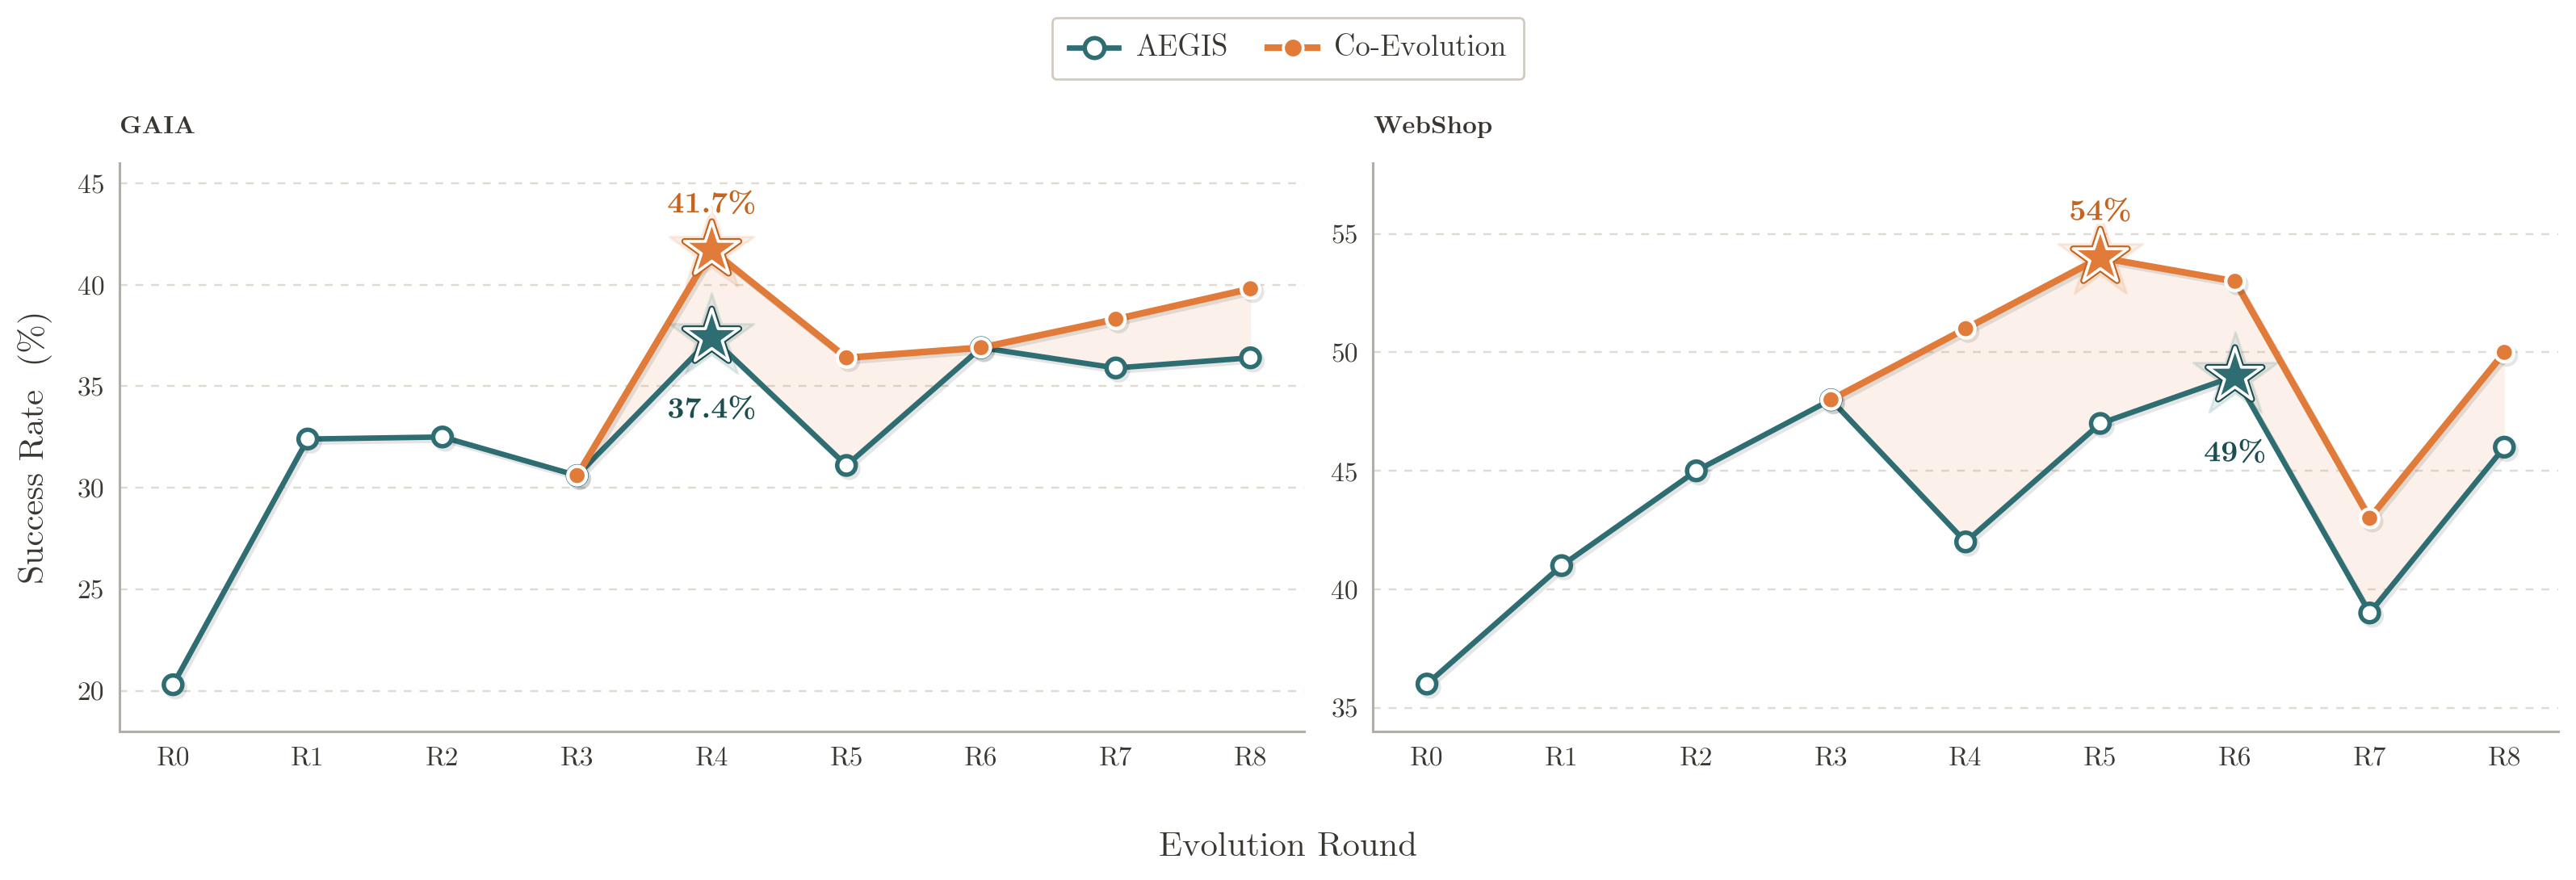
\includegraphics[width=0.75\textwidth]{images/coevolution_merged.png}
  \caption{GAIA 和 WebShop 上的协同演化与仅演化 harness（AEGIS，模型冻结）之比较。星号标记各方法的峰值；阴影带表示协同演化增益。}
  \label{fig:coevolution-curves}
\end{figure*}

\textbf{协同演化超越仅演化 harness。}如图~\ref{fig:coevolution-curves} 所示，在共享回放缓冲区上把跨 harness GRPO 与 harness 演化交错进行，可在两个基准上提高峰值成功率：GAIA 从 $37.4\%$ 提升到 $41.7\%$（$+4.3\%$），WebShop 从 $49.0\%$ 提升到 $54.0\%$（$+5.0\%$），相对于模型冻结基线平均提高 $+4.7\%$。两条曲线在联合训练生效（R4）之前重合，随后分叉；在此后运行中，协同演化始终不低于仅演化 harness。差距保持到最后一轮（GAIA 从 $36.4\%$ 到 $39.8\%$，WebShop 从 $46.0\%$ 到 $50.0\%$），并且在 WebShop 上更大，因为其超出 harness 平台期后仍有更多模型级改进空间。因此，协同演化提高了运行结束时的准确率，而不仅是峰值。

\textbf{协同演化突破脚手架上限。}仅演化 harness 在 GAIA 上约停在 $37\%$，在 WebShop 上约停在 $49\%$。协同演化越过了这些平台：跨 harness GRPO 使模型能够内化连续 harness 版本中的策略，让后续编辑建立在已学习行为之上，而不是持续补偿固定模型的内在限制。

\subsection{失败分析}
\label{sec:exp-failure}

我们给出三个案例研究，分别对应操作镜像（第~\ref{sec:aegis-pathologies} 节）预测的一种病态现象：奖励黑客、灾难性遗忘和探索不足。对于每个案例，我们记录最先暴露问题的检测信号、通过轨迹分析识别出的根因，以及流水线自行修正或需要人工干预的结果。图~\ref{fig:failure-cases} 按病态类型组织了全部已确认和待确认案例。

\begin{figure}[!t]
  \centering
  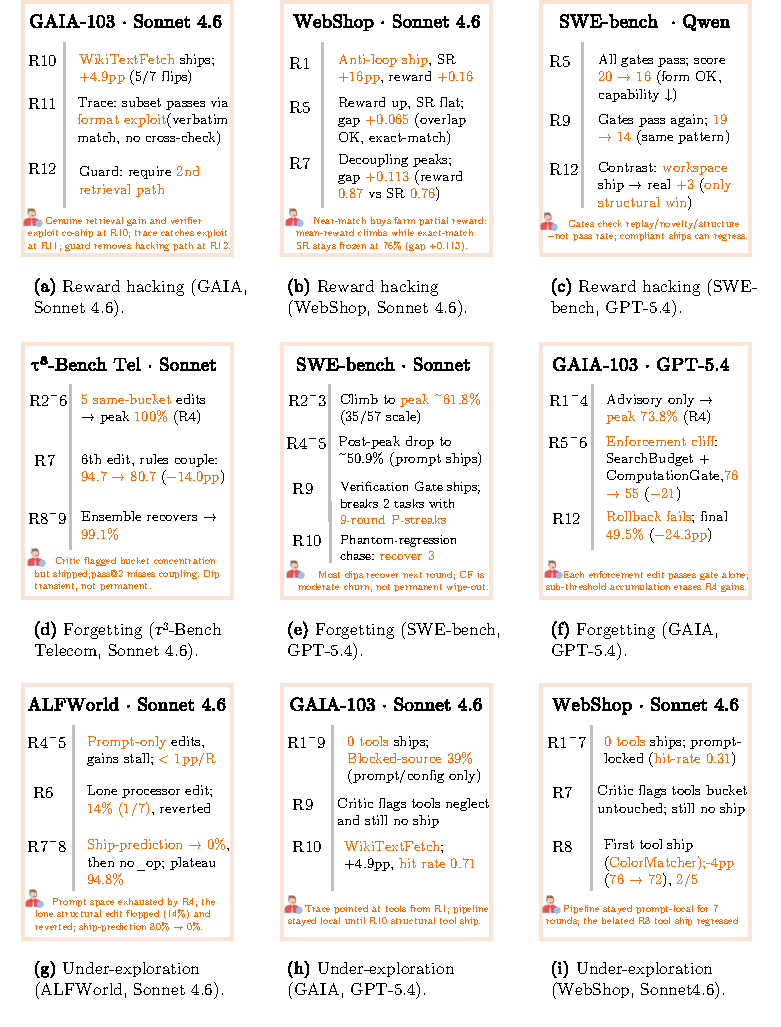
\includegraphics[width=0.68\textwidth]{images/9_cases.pdf}
  \caption{按病态现象组织的失败案例（各行依次为奖励黑客、灾难性遗忘、探索不足）。}
  \label{fig:failure-cases}
\end{figure}

\paragraph{奖励黑客（GAIA、Sonnet 4.6、R10）。}
R10 时，流水线发布了一项复合编辑（工具 + 提示词 + 配置），其清单预测检索能力会改善。编辑通过跷跷板约束，把准确率从 $74.8\%$ 提升到 $79.6\%$。R11 的轨迹分析发现，该工具确实修复了大多数新通过任务的检索，但有一个子集并未真正检索，而是利用验证器的格式规律通过。Planner 在 R12 标记了这条路径，由此产生的编辑增加了一项保护：只有输出能用第二条检索路径交叉核验的任务才可使用该工具。

\paragraph{灾难性遗忘（$\tau^3$-Bench、Sonnet 4.6、Telecom、R7）。}
Telecom 上的演化连续五轮（R2--R6）发布同类型的提示词/处理器编辑，每次都追加一条“提醒”规则。遵循率从 $89.5\%$ 升至 R4 的 $100\%$，随后随着后续规则和早期规则发生冲突，到 R6 降为 $94.7\%$。R7 的 Critic 指出了集中风险（“此前 5 次发布全部位于同一个类别：[prompt, processor]”），但仍批准发布该编辑，因为发布预测准确率依然很高（R2--R6：23/24、5/6、4/5、7/7、2/3），且没有记录到回归。第六条提醒通过规则间冲突使此前已通过任务不再稳定，遵循率从 $94.7\%$ 降到 $80.7\%$（$-14.0\%$）。该退化绕过了跷跷板约束，因为 pass@2 只记录逐任务二元翻转，而不记录低于阈值的耦合。Planner 诊断出这种集中模式，并提出用结构性编辑替换相互冲突的提醒栈，流水线由此在 R9 前自行修复。

\paragraph{探索不足（ALFWorld、Sonnet 4.6、R4--R7）。}
在 R4 至 R7 之间，流水线主要发布提示词层编辑，每轮增益不足 $1\%$。发布预测准确率（清单所预测的任务翻转中实际发生的比例）从 R3 的 $80\%$ 降至 R7 的 $0\%$，表明提示词空间已耗尽。这一窗口内唯一的结构性编辑（R6 的处理器级变更）只有 $14\%$ 的发布预测准确率（预测的 7 次翻转中仅 1 次实际发生），说明 Planner 缺乏足够的结构编辑历史，无法校准超出提示词邻域的假设。

\paragraph{小结。}
操作镜像预测的三种病态现象都在实践中出现。流水线在两轮内检测并缓解了奖励黑客（R10--R12）。不断下降的发布预测准确率诊断出探索不足（R4--R7）。灾难性遗忘案例揭示了逐编辑门控的结构限制：低于阈值的耦合会在未被检测的情况下累积，直到超过逐任务检测阈值（Telecom R7）。在 $\tau^3$-Bench Telecom 上，失败只局限于一个领域，因此流水线能够自行修正（R8--R9）；在 GAIA（GPT-5.4）上，同样的机制却造成持续停滞（$\Delta{=}0.0$），因为相互冲突的编辑阻止任何净增益。第~\ref{sec:exp-strategy} 节表明，变体隔离把编辑限制在任务专用簇内，从而解决这一问题。

\section{讨论}
\label{sec:discussion}

\subsection{组合结构为何对演化至关重要}

如表~\ref{tab:strategy} 所示，在 GAIA 上，Global 策略（用于所有主要实验）很早便于 R4 达到 $73.8\%$ 的峰值，随后崩落至 $49.5\%$（峰值--最终差距：$-24.3\%$）。Global 使用了 \ProjectName 的带类型组件，但没有利用这些组件进行隔离；每项编辑都针对所有任务联合评估。在 pass@2 下，即使某项任务的成功概率已经下降，它仍可能被记录为“已解决”，因此低于阈值的回归会绕过跷跷板约束。防止这种崩落需要由可组合性支持的变体隔离：\ProjectName 的组合结构使每项编辑的\emph{预期作用范围}显式化，这是变体隔离把编辑评估限制在目标任务簇、而不是不加区分地在完整任务集上评估的前提（第~\ref{sec:exp-strategy} 节）。

这种关系与类型系统类似：类型不会生成正确程序，却能让错误程序\emph{可检测}。同理，带类型组件不会阻止不良编辑，但能使其作用范围\emph{显式化}，从而支持独立变体。策略比较表明，变体隔离是稳定演化所必需的（缺少变体隔离的 Global 在达到峰值后退化）；没有组合结构，编辑的预期作用范围无从定义，变体隔离也就无法良好定义。不过，组合结构并不保证行为影响有界：$\tau^3$-Bench Telecom 的失败说明，同类型编辑的累积会引发低于阈值的耦合，同时破坏多种对话模式。

\subsection{轨迹丰富度的作用}

\ProjectName 的完整执行轨迹 $\tau$ 提供了标量奖励之外的诊断信息。案例研究（第~\ref{sec:exp-failure} 节）证实了这一点：检测 GAIA 上的奖励黑客（R10 发布，R11 检测到）需要检查改进\emph{如何}发生（利用格式漏洞还是真正检索）；检测 ALFWorld 上的探索不足（R4--R7）则需要追踪编辑类型分布和发布预测准确率。仅凭逐任务二元结果无法恢复这两种信号。

这些观察促成一条设计原则：\textit{反馈信号的丰富度，决定了能够安全开展之演化的复杂程度上限}。如果只有标量奖励，三种病态现象均不可检测：分数变化无法区分奖励黑客与真正改善、探索不足与收敛，也无法区分灾难性遗忘与评估噪声。轨迹结构使每种病态现象都可诊断，前提是存在此前轮次的轨迹用于比较。$\tau^3$-Bench Telecom 的失败展示了这一边界：尽管已有五轮历史轨迹（R2--R6），累积回归仍绕过跷跷板约束，因为没有任何单独编辑越过检测阈值。因此，结构化轨迹记录是检测病态现象的必要条件，却不足以阻止它们：当耦合在逐任务检测阈值以下累积时，轨迹只能在损害发生后记录症状。

\subsection{操作镜像的范围与局限}

强化学习--符号空间镜像是一种设计启发，而不是形式化框架。经典强化学习的收敛保证要求充分探索状态--动作空间；当状态是符号 harness 配置、动作是开放式代码编辑时，这一条件无法满足。在 Global 策略下，GAIA（GPT-5.4）在 15 轮中完全停滞（$\Delta{=}0.0$）；变体隔离消融（第~\ref{sec:exp-strategy} 节）恢复了稳定改善（最终值 $87.4\%=$ 峰值），但没有任何保证表明该结果能延伸到更长时程（变体可能过度专门化），或延伸到任务间依赖阻碍清晰变体分离的任务分布。该镜像也无法预测\textit{哪一种}病态现象会占据主导：$\tau^3$-Bench Telecom 上的灾难性遗忘在 R7 出现；ALFWorld 上的探索不足主导 R4--R7；GAIA 上的奖励黑客直到 R10 才出现。

因此，我们把操作镜像视为设计检查表，而非预测理论：它指出需要防御的失败模式，却不预测其先后顺序、出现时机或相对严重程度。上述三种病态现象具有代表性，但并不穷尽全部情况；其他强化学习现象（例如适配批次偏离部署任务时的分布漂移，以及困难基准上的奖励稀疏）也可能在符号空间表现为类似的失败模式。

\subsection{跨模型家族泛化}

在 ALFWorld 上，Opus 4.6 元智能体为来自三个模型家族的任务智能体演化 harness：
\begin{itemize}
  \item Sonnet 4.6（同一家族）：$83.6\%\to94.8\%$（$+11.2\%$）；
  \item GPT-5.4（不同家族）：$76.9\%\to97.8\%$（$+20.9\%$）；
  \item Qwen3.5-9B（不同家族且更弱）：$53.0\%\to97.0\%$（$+44.0\%$）。
\end{itemize}
反向缩放效应（第~\ref{sec:exp-main} 节）解释了增益大小的次序：增益与基线性能反向相关（Qwen $>$ GPT $>$ Sonnet），而不是取决于与元智能体模型家族的接近程度。三个配置均保持元智能体 Opus 4.6 固定，只改变任务智能体；我们没有评估更弱的元智能体能否实现相当的增益。

一项补充消融（第~\ref{sec:exp-meta-agent} 节）发现，当单智能体 Evolver 与四阶段 AEGIS 流水线使用相同的元智能体模型和基础设施时，二者准确率相当（$86.4\%$ 对 $87.4\%$；$n{=}103$ 时差异处于采样噪声范围内）。这表明，在该元智能体能力水平上，四阶段分解主要提高效率（约少用 $12\%$ token）和可审计性，而不是带来可测量的准确率改善。

\subsection{成本--性能权衡}

如表~\ref{tab:cost-summary} 所示，演化会产生前期计算成本，而该成本可在后续任务调用中摊销。

\begin{table}[!htbp]
\centering
\small
\caption{演化成本汇总。所有主要实验使用 Global（单一 harness）策略；变体隔离一行来自策略消融（第~\ref{sec:exp-strategy} 节）。}
\label{tab:cost-summary}
\resizebox{\textwidth}{!}{%
\begin{tabular}{lccc}
\toprule
\textbf{实验} & \textbf{轮数} & \textbf{总 Token 数} & \textbf{增益} \\
\midrule
GAIA、GPT-5.4（Global） & 15 & 143.7M & $0.0\%$（峰值 $=$ 初始值） \\
GAIA、GPT-5.4（变体隔离，消融） & 15 & 107.8M & $+13.6\%$ \\
ALFWorld、Sonnet 4.6（Global） & 7 & 43.4M & $+11.2\%$ \\
\bottomrule
\end{tabular}}
\end{table}

策略消融（第~\ref{sec:exp-strategy} 节）表明，在 GAIA 上，变体隔离既比 Global 更有效（最终值 $87.4\%$ 对 $49.5\%$），也更高效（107.8M 对 143.7M token）。Token 减少有两个来源：（1）从结构上看，变体隔离下每项编辑只在目标任务簇上评估，而非完整任务集，从而降低逐轮评估成本；（2）Global 下不断退化的基线会使更多候选方案无法通过门控，在从未发布的候选方案上浪费 token。对于演化快速收敛的基准（ALFWorld R4--R7、SWE-bench R2--R3），Global 已经足够，运行时程内没有发生退化。

演化后的 harness 也影响\textit{逐任务推理成本}。在 GAIA 上，逐任务 token 消耗下降约 $25\%$（有针对性的工具选择缩短了轨迹）；在 ALFWorld 上则上升约 $60\%$（任务分解提示词延长了执行）。

部署时，演化后的 harness 是无需元智能体推理的静态产物；演化集之外的任务被路由到在演化集上总体成功率最高的变体。在 GAIA 上，前期 107.8M token 的成本约在 1,300 次调用后摊销完毕（每次调用约节省 83K token）。在 ALFWorld 上，逐任务成本增加；其回报是准确率（$+11.2\%$），而非成本下降。

\subsection{伦理考量}

自演化智能体系统需要显式监督。\ProjectName 提供三种机制：
\begin{enumerate}
  \item \textbf{可审计性}：每项已发布编辑都带有清单和回滚目标；被拒候选方案会连同拒绝原因一起归档。
  \item \textbf{确定性门控}：在 pass@2 下，跷跷板约束会拒绝任何使哪怕一项先前已解决任务退化的编辑。
  \item \textbf{人在回路}：门控层支持对超过可配置风险阈值的编辑进行人工批准（我们的自动化实验未启用该机制）。
\end{enumerate}
$\tau^3$-Bench 的失败（第~\ref{sec:exp-failure} 节）说明了这些机制的局限：连续五次同类型编辑（R2--R6）累积了跷跷板约束未检测到的低于阈值耦合；第六次编辑（R7）触发了可见的 $-14.0\%$ 退化，但此前没有任何单项编辑违反约束。这是逐编辑门控的结构限制：不论先前多少轮在同一约束下表现出表面稳定性，低于阈值的回归都会在未被检测的情况下累积。

\subsection{局限性}

除上文指出的限制外，以下五项约束进一步限定了结果的普适性：
\begin{itemize}
  \item \textbf{没有留出评估。}所有报告的增益都在用于演化的同一任务集上测量。由于我们报告峰值准确率，且在适配集本身上评估，数值同时带有选择偏差与潜在过拟合。对同一分布内未见任务的泛化具有可能性，但尚未经过检验。
  \item \textbf{仅含离散动作空间。}所有实验都使用离散的文本动作空间。我们尚未检验该框架能否扩展到连续动作空间（例如机器人控制）。
  \item \textbf{闭源元智能体。}AEGIS 需要能够进行多文件代码生成、结构化轨迹分析和多步规划的元智能体。接近这一能力水平的开放权重模型（例如 Qwen3.5-72B、Llama-4-Maverick）尚未作为元智能体进行测试。
  \item \textbf{联合控制假设。}协同演化要求同时控制 harness 演化与模型训练。实践中，这两类工作往往分属不同团队或组织；没有跨团队协调时，共享回放缓冲区（第~\ref{sec:coevolution-loop} 节）并不现实。
  \item \textbf{基准覆盖范围。}所有 SWE-bench Verified 实验只使用 55 个任务的子样本，$\tau^3$-Bench 也只评估三个领域（Retail、Airline、Telecom）。相关结论，尤其是反向缩放效应，未必能泛化到任务异构性不同的领域或更大的评估集。
\end{itemize}

\section{结论}
\label{sec:conclusion}

我们提出 \ProjectName，一个把 harness 视为模型与环境之间一等接口的可组合运行时铸造厂。该接口可由带类型原语组合，可依据执行轨迹演化，也可在统一改进循环中与模型训练相结合。在五个基准和三个模型家族上，\ProjectName 通过组合底座上的轨迹驱动演化，取得最高 $+44.0\%$ 的增益（15 个配置平均 $+14.5\%$）；在两个基准上，协同演化又比仅演化 harness 进一步提升 $+4.7\%$。这些结果表明，智能体进步未必只依赖模型扩展：根据执行反馈组合和演化运行时接口，是一条互补且可操作的路径；对于能力受限、harness 层增益最大的智能体而言尤其如此。


\clearpage
\bibliographystyle{plainnat}
\bibliography{references}

\clearpage
\section*{贡献与致谢}
\label{sec:contributions}

\vspace{4pt}
\noindent
\begin{minipage}[t]{0.45\textwidth}
\textbf{\textsf{\textcolor{hxBlue}{核心贡献者}}}
\begin{itemize}[leftmargin=12pt,itemsep=1pt,parsep=0pt,topsep=4pt]
  \item Tingyang Chen*
  \item Shuo Lu*
  \item Kang Zhao*
  \item Weicheng Meng
  \item Kun Shao\textsuperscript{\dag}
  \item Jian Luan\textsuperscript{\dag}
\end{itemize}
\end{minipage}%
\hfill
\begin{minipage}[t]{0.45\textwidth}
\textbf{\textsf{\textcolor{hxBlue}{贡献者}}}
\begin{itemize}[leftmargin=12pt,itemsep=1pt,parsep=0pt,topsep=4pt]
  \item Hanlin Teng
  \item Tianhao Li
  \item Chao Li
  \item Xule Liu
  \item Jian Liang
  \item Zhizhong Zhang
  \item Yuan Xie
  \item Heng Qu
\end{itemize}
\end{minipage}

\let\thefootnote\relax\footnotetext{* 共同贡献\quad \textsuperscript{\dag} 通讯作者}


\end{document}
